% IEEE conference paper. Build: bash paper/build.sh  (numbers.tex and figures/ are generated from results/).
\documentclass[conference]{IEEEtran}
\IEEEoverridecommandlockouts
\usepackage{cite}
\usepackage{amsmath}
% tectonic = XeTeX: Times via the TeX Gyre Termes OpenType files (text + math)
\usepackage{unicode-math}
\setmainfont{texgyretermes}[Extension=.otf,UprightFont=*-regular,BoldFont=*-bold,ItalicFont=*-italic,BoldItalicFont=*-bolditalic]
\setmathfont{texgyretermes-math.otf}
\usepackage{graphicx}
\usepackage{booktabs}
\usepackage{multirow}
\usepackage{array}
\usepackage{xcolor}
\usepackage{url}
\usepackage{balance}
\usepackage[hidelinks]{hyperref}

% Generated by paper/make_numbers.py from results/*.json. Do not edit by hand.
\providecommand{\TBD}{\textbf{[TBD]}}
\newif\ifHaveTrackXc
\HaveTrackXctrue
\newif\ifHaveEdge
\HaveEdgetrue
\newif\ifHaveEdgeLive
\HaveEdgeLivetrue
\newif\ifHaveJetson
\HaveJetsonfalse
\newif\ifHaveVLMEOne
\HaveVLMEOnetrue
\newif\ifHaveVLMETwo
\HaveVLMETwotrue
\newif\ifHaveVLMEThree
\HaveVLMEThreetrue
\newif\ifHaveVLMEThreeB
\HaveVLMEThreeBtrue
\newif\ifHaveVLMEFive
\HaveVLMEFivetrue
\newif\ifHaveVLMEFour
\HaveVLMEFourtrue
\newif\ifHaveVLM
\HaveVLMtrue
\newif\ifHaveDemo
\HaveDemotrue
\newif\ifHaveHeldout
\HaveHeldouttrue
\newif\ifHaveHeldoutEdge
\HaveHeldoutEdgetrue
\newif\ifHaveTemporalCI
\HaveTemporalCItrue
\newif\ifHaveSafety
\HaveSafetytrue
\newif\ifHaveMultiscene
\HaveMultiscenetrue
\newif\ifHaveWise
\HaveWisetrue
\newif\ifHaveLabelThr
\HaveLabelThrtrue
\newif\ifHaveResSweep
\HaveResSweeptrue
\newif\ifHaveCostLat
\HaveCostLattrue
\newif\ifHaveRobustSel
\HaveRobustSeltrue
\newif\ifHaveBench
\HaveBenchtrue
\newif\ifHaveTrackVone
\HaveTrackVonetrue
\newif\ifHaveTrackVtwo
\HaveTrackVtwotrue
\newif\ifHaveHuman
\HaveHumanfalse
\newcommand{\ApYoloPt}{0.760}
\newcommand{\ApLoYoloPt}{0.751}
\newcommand{\ApHiYoloPt}{0.769}
\newcommand{\ApFiftyYoloPt}{0.947}
\newcommand{\ApFiftyLoYoloPt}{0.942}
\newcommand{\ApFiftyHiYoloPt}{0.953}
\newcommand{\ApSeventyFiveYoloPt}{0.901}
\newcommand{\ApSmallYoloPt}{0.496}
\newcommand{\ApMediumYoloPt}{0.731}
\newcommand{\ApLargeYoloPt}{0.889}
\newcommand{\ArYoloPt}{0.830}
\newcommand{\FoneYoloPt}{0.882}
\newcommand{\FoneLoYoloPt}{0.874}
\newcommand{\FoneHiYoloPt}{0.890}
\newcommand{\PrecYoloPt}{0.878}
\newcommand{\RecYoloPt}{0.886}
\newcommand{\ConfYoloPt}{0.36}
\newcommand{\LamrYoloPt}{0.436}
\newcommand{\FppiYoloPt}{2.33}
\newcommand{\CountMaeYoloPt}{1.69}
\newcommand{\ParamsYoloPt}{2.6}
\newcommand{\GflopsYoloPt}{14.4}
\newcommand{\ApYoloFt}{0.825}
\newcommand{\ApLoYoloFt}{0.818}
\newcommand{\ApHiYoloFt}{0.834}
\newcommand{\ApFiftyYoloFt}{0.963}
\newcommand{\ApFiftyLoYoloFt}{0.959}
\newcommand{\ApFiftyHiYoloFt}{0.967}
\newcommand{\ApSeventyFiveYoloFt}{0.939}
\newcommand{\ApSmallYoloFt}{0.552}
\newcommand{\ApMediumYoloFt}{0.810}
\newcommand{\ApLargeYoloFt}{0.910}
\newcommand{\ArYoloFt}{0.875}
\newcommand{\FoneYoloFt}{0.891}
\newcommand{\FoneLoYoloFt}{0.882}
\newcommand{\FoneHiYoloFt}{0.900}
\newcommand{\PrecYoloFt}{0.833}
\newcommand{\RecYoloFt}{0.957}
\newcommand{\ConfYoloFt}{0.24}
\newcommand{\LamrYoloFt}{0.354}
\newcommand{\FppiYoloFt}{3.62}
\newcommand{\CountMaeYoloFt}{3.01}
\newcommand{\ParamsYoloFt}{2.5}
\newcommand{\GflopsYoloFt}{13.6}
\newcommand{\ApRfPt}{0.382}
\newcommand{\ApLoRfPt}{0.366}
\newcommand{\ApHiRfPt}{0.401}
\newcommand{\ApFiftyRfPt}{0.705}
\newcommand{\ApFiftyLoRfPt}{0.684}
\newcommand{\ApFiftyHiRfPt}{0.723}
\newcommand{\ApSeventyFiveRfPt}{0.357}
\newcommand{\ApSmallRfPt}{0.199}
\newcommand{\ApMediumRfPt}{0.285}
\newcommand{\ApLargeRfPt}{0.699}
\newcommand{\ArRfPt}{0.514}
\newcommand{\FoneRfPt}{0.658}
\newcommand{\FoneLoRfPt}{0.640}
\newcommand{\FoneHiRfPt}{0.677}
\newcommand{\PrecRfPt}{0.694}
\newcommand{\RecRfPt}{0.626}
\newcommand{\ConfRfPt}{0.31}
\newcommand{\LamrRfPt}{0.711}
\newcommand{\FppiRfPt}{5.23}
\newcommand{\CountMaeRfPt}{2.63}
\newcommand{\ParamsRfPt}{30.5}
\newcommand{\GflopsRfPt}{31.9}
\newcommand{\ApRfFt}{0.725}
\newcommand{\ApLoRfFt}{0.714}
\newcommand{\ApHiRfFt}{0.738}
\newcommand{\ApFiftyRfFt}{0.943}
\newcommand{\ApFiftyLoRfFt}{0.937}
\newcommand{\ApFiftyHiRfFt}{0.950}
\newcommand{\ApSeventyFiveRfFt}{0.838}
\newcommand{\ApSmallRfFt}{0.298}
\newcommand{\ApMediumRfFt}{0.691}
\newcommand{\ApLargeRfFt}{0.898}
\newcommand{\ArRfFt}{0.808}
\newcommand{\FoneRfFt}{0.885}
\newcommand{\FoneLoRfFt}{0.876}
\newcommand{\FoneHiRfFt}{0.895}
\newcommand{\PrecRfFt}{0.899}
\newcommand{\RecRfFt}{0.872}
\newcommand{\ConfRfFt}{0.46}
\newcommand{\LamrRfFt}{0.411}
\newcommand{\FppiRfFt}{1.85}
\newcommand{\CountMaeRfFt}{1.54}
\newcommand{\ParamsRfFt}{30.5}
\newcommand{\GflopsRfFt}{97.3}
\newcommand{\ApTrainYoloPt}{0.788}
\newcommand{\ApValidYoloPt}{0.800}
\newcommand{\ApTestYoloPt}{0.760}
\newcommand{\ApTrainYoloFt}{0.920}
\newcommand{\ApValidYoloFt}{0.854}
\newcommand{\ApTestYoloFt}{0.825}
\newcommand{\ApTrainRfPt}{0.531}
\newcommand{\ApValidRfPt}{0.503}
\newcommand{\ApTestRfPt}{0.382}
\newcommand{\ApTrainRfFt}{0.847}
\newcommand{\ApValidRfFt}{0.801}
\newcommand{\ApTestRfFt}{0.725}
\newcommand{\GapYoloFt}{$+$0.094}
\newcommand{\GapPtYoloFt}{$+$0.028}
\newcommand{\ExcessYoloFt}{$+$0.066}
\newcommand{\GapValidYoloFt}{$+$0.066}
\newcommand{\GapRfFt}{$+$0.122}
\newcommand{\GapPtRfFt}{$+$0.148}
\newcommand{\ExcessRfFt}{$-$0.026}
\newcommand{\GapValidRfFt}{$+$0.046}
\newcommand{\DeltaFtFt}{$+$0.099}
\newcommand{\DeltaLoFtFt}{$+$0.092}
\newcommand{\DeltaHiFtFt}{$+$0.107}
\newcommand{\PvalFtFt}{$p<0.001$}
\newcommand{\DeltaYoloFtPt}{$+$0.065}
\newcommand{\DeltaLoYoloFtPt}{$+$0.060}
\newcommand{\DeltaHiYoloFtPt}{$+$0.071}
\newcommand{\PvalYoloFtPt}{$p<0.001$}
\newcommand{\DeltaRfFtPt}{$+$0.343}
\newcommand{\DeltaLoRfFtPt}{$+$0.331}
\newcommand{\DeltaHiRfFtPt}{$+$0.354}
\newcommand{\PvalRfFtPt}{$p<0.001$}
\newcommand{\DeltaYoloPtRfFt}{$+$0.034}
\newcommand{\DeltaLoYoloPtRfFt}{$+$0.026}
\newcommand{\DeltaHiYoloPtRfFt}{$+$0.042}
\newcommand{\PvalYoloPtRfFt}{$p<0.001$}
\newcommand{\ImgsTrain}{720}
\newcommand{\BoxesTrain}{12{,}024}
\newcommand{\ImgsValid}{180}
\newcommand{\BoxesValid}{3{,}371}
\newcommand{\ImgsTest}{182}
\newcommand{\BoxesTest}{3{,}441}
\newcommand{\BoxesTotal}{18{,}836}
\newcommand{\BoxesPerFrameTest}{18.9}
\newcommand{\XcPass}{50}
\newcommand{\XcTotal}{50}
\newcommand{\XcApMaxDiff}{0.0012}
\newcommand{\XcUltraDiff}{0.010}
\newcommand{\XtPass}{4}
\newcommand{\XtTotal}{4}
\newcommand{\LatYoloBase}{5.31}
\newcommand{\LatPnYoloBase}{5.56}
\newcommand{\FpsYoloBase}{188}
\newcommand{\LatApYoloBase}{0.827}
\newcommand{\LatYoloHalf}{4.52}
\newcommand{\LatPnYoloHalf}{4.86}
\newcommand{\FpsYoloHalf}{221}
\newcommand{\LatApYoloHalf}{0.821}
\newcommand{\LatYoloNmsFree}{4.33}
\newcommand{\LatPnYoloNmsFree}{4.73}
\newcommand{\FpsYoloNmsFree}{231}
\newcommand{\LatApYoloNmsFree}{0.803}
\newcommand{\LatYoloNmsFreeFast}{3.44}
\newcommand{\LatPnYoloNmsFreeFast}{3.72}
\newcommand{\FpsYoloNmsFreeFast}{290}
\newcommand{\LatApYoloNmsFreeFast}{0.808}
\newcommand{\LatYoloDep}{3.68}
\newcommand{\LatPnYoloDep}{4.04}
\newcommand{\FpsYoloDep}{272}
\newcommand{\LatApYoloDep}{0.825}
\newcommand{\LatRfBase}{21.33}
\newcommand{\LatPnRfBase}{22.41}
\newcommand{\FpsRfBase}{47}
\newcommand{\LatApRfBase}{0.727}
\newcommand{\LatRfTs}{20.14}
\newcommand{\LatPnRfTs}{20.83}
\newcommand{\FpsRfTs}{50}
\newcommand{\LatApRfTs}{0.727}
\newcommand{\LatRfHalf}{11.42}
\newcommand{\LatPnRfHalf}{12.36}
\newcommand{\FpsRfHalf}{88}
\newcommand{\LatApRfHalf}{0.726}
\newcommand{\LatRfHalfTs}{9.77}
\newcommand{\LatPnRfHalfTs}{10.54}
\newcommand{\FpsRfHalfTs}{102}
\newcommand{\LatApRfHalfTs}{0.725}
\newcommand{\LatRfDep}{7.89}
\newcommand{\LatPnRfDep}{8.73}
\newcommand{\FpsRfDep}{127}
\newcommand{\LatApRfDep}{0.725}
\newcommand{\SpeedupYolo}{1.4}
\newcommand{\SpeedupRf}{2.7}
\newcommand{\LatRatio}{2.1}
\newcommand{\NmsFreeApLoss}{0.017}
\newcommand{\TbYoloPtFused}{0.760}
\newcommand{\TbYoloPtRfL}{0.696}
\newcommand{\TbYoloPtYx}{0.722}
\newcommand{\TbYoloFtFused}{0.825}
\newcommand{\TbYoloFtRfL}{0.726}
\newcommand{\TbYoloFtYx}{0.773}
\newcommand{\TbRfPtFused}{0.382}
\newcommand{\TbRfPtRfL}{0.448}
\newcommand{\TbRfPtYx}{0.324}
\newcommand{\TbRfFtFused}{0.725}
\newcommand{\TbRfFtRfL}{0.731}
\newcommand{\TbRfFtYx}{0.630}
\newcommand{\LabelsFused}{3{,}441}
\newcommand{\LabelsRfL}{2{,}587}
\newcommand{\LabelsYx}{4{,}226}
\newcommand{\TbGapRfL}{$-$0.005}
\newcommand{\TbGapYx}{$+$0.143}
\newcommand{\BtHotaYoloDef}{0.715}
\newcommand{\BtMotaYoloDef}{0.731}
\newcommand{\BtIdfYoloDef}{0.774}
\newcommand{\BtDetaYoloDef}{0.713}
\newcommand{\BtAssaYoloDef}{0.719}
\newcommand{\BtIdswYoloDef}{40}
\newcommand{\BtIdsYoloDef}{115}
\newcommand{\BtHotaYoloTun}{0.746}
\newcommand{\BtMotaYoloTun}{0.770}
\newcommand{\BtIdfYoloTun}{0.805}
\newcommand{\BtDetaYoloTun}{0.737}
\newcommand{\BtAssaYoloTun}{0.759}
\newcommand{\BtIdswYoloTun}{42}
\newcommand{\BtIdsYoloTun}{138}
\newcommand{\BtMinConfYolo}{0.2}
\newcommand{\BtBufferYolo}{30}
\newcommand{\BtConfirmYolo}{3}
\newcommand{\BtHotaRfDef}{0.644}
\newcommand{\BtMotaRfDef}{0.560}
\newcommand{\BtIdfRfDef}{0.721}
\newcommand{\BtDetaRfDef}{0.623}
\newcommand{\BtAssaRfDef}{0.670}
\newcommand{\BtIdswRfDef}{69}
\newcommand{\BtIdsRfDef}{123}
\newcommand{\BtHotaRfTun}{0.757}
\newcommand{\BtMotaRfTun}{0.788}
\newcommand{\BtIdfRfTun}{0.829}
\newcommand{\BtDetaRfTun}{0.732}
\newcommand{\BtAssaRfTun}{0.786}
\newcommand{\BtIdswRfTun}{60}
\newcommand{\BtIdsRfTun}{145}
\newcommand{\BtMinConfRf}{0.5}
\newcommand{\BtBufferRf}{15}
\newcommand{\BtConfirmRf}{1}
\newcommand{\BtGtIds}{112}
\newcommand{\BtTunGap}{$-$0.010}
\newcommand{\BtDefGap}{$+$0.071}
\newcommand{\GridSize}{4{,}344}
\newcommand{\GtTracks}{169}
\newcommand{\GtFrames}{1{,}798}
\newcommand{\GtBuffer}{120}
\newcommand{\TcYoloSortBtGt}{0.749}
\newcommand{\TcbYoloSortBtGt}{0.749}
\newcommand{\TcYoloSortOcGt}{0.653}
\newcommand{\TcbYoloSortOcGt}{0.653}
\newcommand{\TcYoloByteBtGt}{0.758}
\newcommand{\TcbYoloByteBtGt}{\textbf{0.758}}
\newcommand{\TcYoloByteOcGt}{0.653}
\newcommand{\TcbYoloByteOcGt}{0.653}
\newcommand{\TcYoloOcsortBtGt}{0.758}
\newcommand{\TcbYoloOcsortBtGt}{0.758}
\newcommand{\TcYoloOcsortOcGt}{0.648}
\newcommand{\TcbYoloOcsortOcGt}{0.648}
\newcommand{\TcYoloCbiouBtGt}{0.738}
\newcommand{\TcbYoloCbiouBtGt}{0.738}
\newcommand{\TcYoloCbiouOcGt}{0.659}
\newcommand{\TcbYoloCbiouOcGt}{0.659}
\newcommand{\TcYoloBotsortBtGt}{0.737}
\newcommand{\TcbYoloBotsortBtGt}{0.737}
\newcommand{\TcYoloBotsortOcGt}{0.656}
\newcommand{\TcbYoloBotsortOcGt}{0.656}
\newcommand{\TcYoloMcbyteBtGt}{0.751}
\newcommand{\TcbYoloMcbyteBtGt}{0.751}
\newcommand{\TcYoloMcbyteOcGt}{0.661}
\newcommand{\TcbYoloMcbyteOcGt}{\textbf{0.661}}
\newcommand{\TcRfSortBtGt}{0.734}
\newcommand{\TcbRfSortBtGt}{0.734}
\newcommand{\TcRfSortOcGt}{0.629}
\newcommand{\TcbRfSortOcGt}{0.629}
\newcommand{\TcRfByteBtGt}{0.739}
\newcommand{\TcbRfByteBtGt}{0.739}
\newcommand{\TcRfByteOcGt}{0.633}
\newcommand{\TcbRfByteOcGt}{0.633}
\newcommand{\TcRfOcsortBtGt}{0.738}
\newcommand{\TcbRfOcsortBtGt}{0.738}
\newcommand{\TcRfOcsortOcGt}{0.629}
\newcommand{\TcbRfOcsortOcGt}{0.629}
\newcommand{\TcRfCbiouBtGt}{0.741}
\newcommand{\TcbRfCbiouBtGt}{0.741}
\newcommand{\TcRfCbiouOcGt}{0.641}
\newcommand{\TcbRfCbiouOcGt}{0.641}
\newcommand{\TcRfBotsortBtGt}{0.747}
\newcommand{\TcbRfBotsortBtGt}{\textbf{0.747}}
\newcommand{\TcRfBotsortOcGt}{0.635}
\newcommand{\TcbRfBotsortOcGt}{0.635}
\newcommand{\TcRfMcbyteBtGt}{0.743}
\newcommand{\TcbRfMcbyteBtGt}{0.743}
\newcommand{\TcRfMcbyteOcGt}{0.643}
\newcommand{\TcbRfMcbyteOcGt}{\textbf{0.643}}
\newcommand{\TcWinsBtGt}{4}
\newcommand{\TcMeanYoloBtGt}{0.748}
\newcommand{\TcMeanRfBtGt}{0.740}
\newcommand{\TcSpreadBtGt}{0.02}
\newcommand{\TcWinsOcGt}{6}
\newcommand{\TcMeanYoloOcGt}{0.655}
\newcommand{\TcMeanRfOcGt}{0.635}
\newcommand{\TcSpreadOcGt}{0.01}
\newcommand{\TcWinsAll}{10}
\newcommand{\TcPairs}{12}
\newcommand{\TcMaxGap}{0.02}
\newcommand{\AnUniqueYolo}{176}
\newcommand{\AnRawYolo}{209}
\newcommand{\AnMeanYolo}{16.2}
\newcommand{\AnMaxYolo}{23}
\newcommand{\AnDwellMedYolo}{1.5}
\newcommand{\AnDwellPnYolo}{6.1}
\newcommand{\AnOverYolo}{$+$4\%}
\newcommand{\AnGtUnique}{169}
\newcommand{\AnUniqueRf}{181}
\newcommand{\AnRawRf}{219}
\newcommand{\AnMeanRf}{14.7}
\newcommand{\AnMaxRf}{20}
\newcommand{\AnDwellMedRf}{1.3}
\newcommand{\AnDwellPnRf}{4.9}
\newcommand{\AnOverRf}{$+$7\%}
\newcommand{\MsWAp}{0.30}
\newcommand{\MsApYolo}{0.825}
\newcommand{\MsNApYolo}{1.00}
\newcommand{\MsApRf}{0.725}
\newcommand{\MsNApRf}{0.88}
\newcommand{\MsWBias}{0.10}
\newcommand{\MsBiasYolo}{0.726}
\newcommand{\MsNBiasYolo}{1.00}
\newcommand{\MsBiasRf}{0.630}
\newcommand{\MsNBiasRf}{0.87}
\newcommand{\MsWHota}{0.25}
\newcommand{\MsHotaYolo}{0.702}
\newcommand{\MsNHotaYolo}{1.00}
\newcommand{\MsHotaRf}{0.688}
\newcommand{\MsNHotaRf}{0.98}
\newcommand{\MsWLat}{0.20}
\newcommand{\MsLatYolo}{3.68}
\newcommand{\MsNLatYolo}{1.00}
\newcommand{\MsLatRf}{7.89}
\newcommand{\MsNLatRf}{0.47}
\newcommand{\MsWGflops}{0.10}
\newcommand{\MsGflopsYolo}{13.6}
\newcommand{\MsNGflopsYolo}{1.00}
\newcommand{\MsGflopsRf}{97.3}
\newcommand{\MsNGflopsRf}{0.14}
\newcommand{\MsWParams}{0.05}
\newcommand{\MsParamsYolo}{2.5}
\newcommand{\MsNParamsYolo}{1.00}
\newcommand{\MsParamsRf}{30.5}
\newcommand{\MsNParamsRf}{0.08}
\newcommand{\MsCritWins}{6}
\newcommand{\MsCritN}{6}
\newcommand{\MsScoreYolo}{1.00}
\newcommand{\MsTrackWinsYolo}{10/12}
\newcommand{\MsScoreRf}{0.71}
\newcommand{\MsTrackWinsRf}{2/12}
\newcommand{\MsAltAccRf}{0.88}
\newcommand{\MsAltAccWin}{YOLO26n}
\newcommand{\MsAltSpeedRf}{0.47}
\newcommand{\MsAltSpeedWin}{YOLO26n}
\newcommand{\MsAltTrackRf}{0.98}
\newcommand{\MsAltTrackWin}{YOLO26n}
\newcommand{\MsAltEqualRf}{0.57}
\newcommand{\MsAltEqualWin}{YOLO26n}
\newcommand{\MsAltBiasRf}{0.70}
\newcommand{\MsAltBiasWin}{YOLO26n}
\newcommand{\MsWinner}{YOLO26n}
\newcommand{\MsRobust}{yes}
\newcommand{\MsNumAlt}{5}
\newcommand{\OnnxHiAp}{0.827}
\newcommand{\OnnxHiApFifty}{0.963}
\newcommand{\OnnxHiApSmall}{0.552}
\newcommand{\OnnxHiAr}{0.877}
\newcommand{\OnnxHiCpuMs}{31}
\newcommand{\OnnxMidAp}{0.794}
\newcommand{\OnnxMidApFifty}{0.959}
\newcommand{\OnnxMidApSmall}{0.505}
\newcommand{\OnnxMidAr}{0.847}
\newcommand{\OnnxMidCpuMs}{41}
\newcommand{\OnnxLoAp}{0.682}
\newcommand{\OnnxLoApFifty}{0.925}
\newcommand{\OnnxLoApSmall}{0.295}
\newcommand{\OnnxLoAr}{0.746}
\newcommand{\OnnxLoCpuMs}{19}
\newcommand{\OnnxParityDiff}{0.0019}
\newcommand{\OnnxParityPt}{0.825}
\newcommand{\CpOnePeople}{257}
\newcommand{\CpOneRaw}{431}
\newcommand{\CpOneKept}{307}
\newcommand{\CpOneAttr}{244}
\newcommand{\CpOneMean}{8.5}
\newcommand{\CpOnePeak}{16}
\newcommand{\CpOneDwell}{3.6}
\newcommand{\CpOneCross}{73}
\newcommand{\CpOneCrossRl}{71}
\newcommand{\CpOneCrossLr}{2}
\newcommand{\CpOneMale}{143}
\newcommand{\CpOneFemale}{78}
\newcommand{\CpOneGUnsure}{23}
\newcommand{\CpOneUniform}{191}
\newcommand{\CpOneNonUniform}{38}
\newcommand{\CpOneDUnsure}{15}
\newcommand{\CpOneSeconds}{200}
\newcommand{\CpOneFps}{53}
\newcommand{\CpOneStitch}{50}
\newcommand{\CpTwoPeople}{307}
\newcommand{\CpTwoRaw}{670}
\newcommand{\CpTwoKept}{458}
\newcommand{\CpTwoAttr}{286}
\newcommand{\CpTwoMean}{8.5}
\newcommand{\CpTwoPeak}{18}
\newcommand{\CpTwoDwell}{3.1}
\newcommand{\CpTwoCross}{92}
\newcommand{\CpTwoCrossRl}{87}
\newcommand{\CpTwoCrossLr}{5}
\newcommand{\CpTwoMale}{117}
\newcommand{\CpTwoFemale}{144}
\newcommand{\CpTwoGUnsure}{25}
\newcommand{\CpTwoUniform}{263}
\newcommand{\CpTwoNonUniform}{15}
\newcommand{\CpTwoDUnsure}{8}
\newcommand{\CpTwoSeconds}{200}
\newcommand{\CpTwoFps}{49}
\newcommand{\CpTwoStitch}{219}
\newcommand{\PrUniAcc}{0.90}
\newcommand{\PrUniLo}{0.80}
\newcommand{\PrUniHi}{0.95}
\newcommand{\PrUniCorrect}{61}
\newcommand{\PrUniAnswered}{68}
\newcommand{\PrUniCov}{93\%}
\newcommand{\PrUniTrackAcc}{0.83}
\newcommand{\PrUniTrackCorrect}{60}
\newcommand{\PrUniTrackAnswered}{72}
\newcommand{\PrUniCv}{0.93}
\newcommand{\PrUniTrackOne}{0.89}
\newcommand{\PrUniTrackTwo}{0.77}
\newcommand{\PrGenAcc}{0.87}
\newcommand{\PrGenLo}{0.76}
\newcommand{\PrGenHi}{0.93}
\newcommand{\PrGenCorrect}{58}
\newcommand{\PrGenAnswered}{67}
\newcommand{\PrGenCov}{88\%}
\newcommand{\PrGenTrackAcc}{0.80}
\newcommand{\PrGenTrackCorrect}{57}
\newcommand{\PrGenTrackAnswered}{71}
\newcommand{\PrGenCv}{0.93}
\newcommand{\PrGenTrackOne}{0.83}
\newcommand{\PrGenTrackTwo}{0.78}
\newcommand{\EdHotaHiSOne}{0.746}
\newcommand{\EdMotaHiSOne}{0.758}
\newcommand{\EdIdfHiSOne}{0.806}
\newcommand{\EdHotaFullHiSOne}{0.740}
\newcommand{\EdUniqueHiSOne}{181}
\newcommand{\EdGtUniqueHiSOne}{169}
\newcommand{\EdFpsHiSOne}{59.9}
\newcommand{\EdStrideHiSOne}{1}
\newcommand{\EdDetMsHiSOne}{32.5}
\newcommand{\EdTrkMsHiSOne}{0.97}
\newcommand{\EdAnaMsHiSOne}{0.16}
\newcommand{\EdLoopMsHiSOne}{33.6}
\newcommand{\EdHotaHiSTwo}{0.743}
\newcommand{\EdMotaHiSTwo}{0.753}
\newcommand{\EdIdfHiSTwo}{0.806}
\newcommand{\EdHotaFullHiSTwo}{0.733}
\newcommand{\EdUniqueHiSTwo}{164}
\newcommand{\EdGtUniqueHiSTwo}{165}
\newcommand{\EdFpsHiSTwo}{30.0}
\newcommand{\EdStrideHiSTwo}{2}
\newcommand{\EdDetMsHiSTwo}{32.6}
\newcommand{\EdTrkMsHiSTwo}{0.94}
\newcommand{\EdAnaMsHiSTwo}{0.16}
\newcommand{\EdLoopMsHiSTwo}{34.2}
\newcommand{\EdHotaHiSFour}{0.735}
\newcommand{\EdMotaHiSFour}{0.736}
\newcommand{\EdIdfHiSFour}{0.796}
\newcommand{\EdHotaFullHiSFour}{0.731}
\newcommand{\EdUniqueHiSFour}{160}
\newcommand{\EdGtUniqueHiSFour}{168}
\newcommand{\EdFpsHiSFour}{15.0}
\newcommand{\EdStrideHiSFour}{4}
\newcommand{\EdDetMsHiSFour}{33.0}
\newcommand{\EdTrkMsHiSFour}{0.88}
\newcommand{\EdAnaMsHiSFour}{0.22}
\newcommand{\EdLoopMsHiSFour}{34.0}
\newcommand{\EdHotaMidSFour}{0.726}
\newcommand{\EdMotaMidSFour}{0.754}
\newcommand{\EdIdfMidSFour}{0.794}
\newcommand{\EdHotaFullMidSFour}{0.729}
\newcommand{\EdUniqueMidSFour}{144}
\newcommand{\EdGtUniqueMidSFour}{168}
\newcommand{\EdFpsMidSFour}{15.0}
\newcommand{\EdStrideMidSFour}{4}
\newcommand{\EdDetMsMidSFour}{17.6}
\newcommand{\EdTrkMsMidSFour}{0.85}
\newcommand{\EdAnaMsMidSFour}{0.17}
\newcommand{\EdLoopMsMidSFour}{18.6}
\newcommand{\EdHotaLoSFour}{0.699}
\newcommand{\EdMotaLoSFour}{0.718}
\newcommand{\EdIdfLoSFour}{0.785}
\newcommand{\EdHotaFullLoSFour}{0.664}
\newcommand{\EdUniqueLoSFour}{125}
\newcommand{\EdGtUniqueLoSFour}{168}
\newcommand{\EdFpsLoSFour}{15.0}
\newcommand{\EdStrideLoSFour}{4}
\newcommand{\EdDetMsLoSFour}{9.6}
\newcommand{\EdTrkMsLoSFour}{0.79}
\newcommand{\EdAnaMsLoSFour}{0.13}
\newcommand{\EdLoopMsLoSFour}{10.5}
\newcommand{\EdProvider}{CPUExecutionProvider}
\newcommand{\EdRefHota}{0.746}
\newcommand{\EdRefGap}{$+$0.000}
\newcommand{\EdLiveFrames}{1{,}602}
\newcommand{\EdLiveDropped}{197}
\newcommand{\EdLivePublished}{1{,}798}
\newcommand{\EdLiveFps}{47.1}
\newcommand{\EdLiveDetMs}{14.1}
\newcommand{\EdLiveLoopMs}{15.3}
\newcommand{\EdLiveUnique}{152}
\newcommand{\EdLiveBackend}{ultralytics}
\newcommand{\EoFrames}{182}
\newcommand{\EoGtMin}{13}
\newcommand{\EoGtMax}{24}
\newcommand{\EoMaeA}{2.97}
\newcommand{\EoMaeLoA}{2.60}
\newcommand{\EoMaeHiA}{3.37}
\newcommand{\EoRmseA}{4.04}
\newcommand{\EoBiasA}{$+$2.84}
\newcommand{\EoExactA}{0.13}
\newcommand{\EoWithinA}{0.52}
\newcommand{\EoRA}{0.48}
\newcommand{\EoParseA}{0.00}
\newcommand{\EoMaeB}{7.91}
\newcommand{\EoMaeLoB}{7.45}
\newcommand{\EoMaeHiB}{8.36}
\newcommand{\EoRmseB}{8.50}
\newcommand{\EoBiasB}{$-$7.91}
\newcommand{\EoExactB}{0.02}
\newcommand{\EoWithinB}{0.06}
\newcommand{\EoRB}{$-$0.35}
\newcommand{\EoParseB}{0.00}
\newcommand{\EoCopyB}{0.00}
\newcommand{\EoMaeBsys}{3.16}
\newcommand{\EoMaeLoBsys}{2.82}
\newcommand{\EoMaeHiBsys}{3.50}
\newcommand{\EoRmseBsys}{3.96}
\newcommand{\EoBiasBsys}{$-$2.29}
\newcommand{\EoExactBsys}{0.12}
\newcommand{\EoWithinBsys}{0.48}
\newcommand{\EoRBsys}{0.19}
\newcommand{\EoParseBsys}{0.00}
\newcommand{\EoCopyBsys}{0.03}
\newcommand{\EoMaeC}{2.97}
\newcommand{\EoMaeLoC}{2.60}
\newcommand{\EoMaeHiC}{3.37}
\newcommand{\EoRmseC}{4.04}
\newcommand{\EoBiasC}{$+$2.84}
\newcommand{\EoExactC}{0.13}
\newcommand{\EoWithinC}{0.52}
\newcommand{\EoRC}{0.48}
\newcommand{\EoParseC}{0.00}
\newcommand{\EoCopyC}{1.00}
\newcommand{\EoMaeD}{2.97}
\newcommand{\EoMaeLoD}{2.60}
\newcommand{\EoMaeHiD}{3.37}
\newcommand{\EoRmseD}{4.04}
\newcommand{\EoBiasD}{$+$2.84}
\newcommand{\EoExactD}{0.13}
\newcommand{\EoWithinD}{0.52}
\newcommand{\EoRD}{0.48}
\newcommand{\EoParseD}{0.00}
\newcommand{\EoCopyD}{1.00}
\newcommand{\EoDeltaBC}{$+$4.93}
\newcommand{\EoDeltaLoBC}{$+$4.32}
\newcommand{\EoDeltaHiBC}{$+$5.61}
\newcommand{\EoPvalBC}{$p<0.001$}
\newcommand{\EoDeltaAC}{$+$0.00}
\newcommand{\EoDeltaLoAC}{$+$0.00}
\newcommand{\EoDeltaHiAC}{$+$0.00}
\newcommand{\EoPvalAC}{$p=1.00$}
\newcommand{\EoDeltaCD}{$+$0.00}
\newcommand{\EoDeltaLoCD}{$+$0.00}
\newcommand{\EoDeltaHiCD}{$+$0.00}
\newcommand{\EoPvalCD}{$p=1.00$}
\newcommand{\EoDeltaBBsys}{$+$4.74}
\newcommand{\EoDeltaLoBBsys}{$+$4.28}
\newcommand{\EoDeltaHiBBsys}{$+$5.19}
\newcommand{\EoPvalBBsys}{$p<0.001$}
\newcommand{\EoStratNLow}{0}
\newcommand{\EoStratLowA}{--}
\newcommand{\EoStratLowB}{--}
\newcommand{\EoStratLowC}{--}
\newcommand{\EoStratNMid}{136}
\newcommand{\EoStratMidA}{3.39}
\newcommand{\EoStratMidB}{6.79}
\newcommand{\EoStratMidC}{3.39}
\newcommand{\EoStratNHigh}{46}
\newcommand{\EoStratHighA}{1.74}
\newcommand{\EoStratHighB}{11.20}
\newcommand{\EoStratHighC}{1.74}
\newcommand{\EtVlmAccUni}{0.83}
\newcommand{\EtVlmLoUni}{0.74}
\newcommand{\EtVlmHiUni}{0.90}
\newcommand{\EtVlmCovUni}{100\%}
\newcommand{\EtVlmCorrectUni}{66}
\newcommand{\EtVlmAnsweredUni}{79}
\newcommand{\EtProbeAccUni}{0.83}
\newcommand{\EtProbeLoUni}{0.73}
\newcommand{\EtProbeHiUni}{0.90}
\newcommand{\EtProbeCovUni}{91\%}
\newcommand{\EtProbeCorrectUni}{60}
\newcommand{\EtProbeAnsweredUni}{72}
\newcommand{\EtMcPUni}{$p=1.00$}
\newcommand{\EtMcNUni}{72}
\newcommand{\EtMcPwUni}{2}
\newcommand{\EtMcVwUni}{2}
\newcommand{\EtVlmAccGen}{0.79}
\newcommand{\EtVlmLoGen}{0.69}
\newcommand{\EtVlmHiGen}{0.86}
\newcommand{\EtVlmCovGen}{99\%}
\newcommand{\EtVlmCorrectGen}{63}
\newcommand{\EtVlmAnsweredGen}{80}
\newcommand{\EtProbeAccGen}{0.80}
\newcommand{\EtProbeLoGen}{0.70}
\newcommand{\EtProbeHiGen}{0.88}
\newcommand{\EtProbeCovGen}{88\%}
\newcommand{\EtProbeCorrectGen}{57}
\newcommand{\EtProbeAnsweredGen}{71}
\newcommand{\EtMcPGen}{$p=1.00$}
\newcommand{\EtMcNGen}{70}
\newcommand{\EtMcPwGen}{11}
\newcommand{\EtMcVwGen}{12}
\newcommand{\EtJsonValid}{1.00}
\newcommand{\EthSelFrame}{0.62}
\newcommand{\EthSelLoFrame}{0.48}
\newcommand{\EthSelHiFrame}{0.75}
\newcommand{\EthSelToolFrame}{0.83}
\newcommand{\EthArgFrame}{0.55}
\newcommand{\EthArgLoFrame}{0.38}
\newcommand{\EthArgHiFrame}{0.72}
\newcommand{\EthArgLenFrame}{0.66}
\newcommand{\EthArgGivenFrame}{0.67}
\newcommand{\EthFpFrame}{0.75}
\newcommand{\EthMissFrame}{0.00}
\newcommand{\EthJsonFrame}{1.00}
\newcommand{\EthLatFrame}{0.27}
\newcommand{\EthSetAlertArgFrame}{0.31}
\newcommand{\EthLineArgFrame}{0.60}
\newcommand{\EthSelText}{0.91}
\newcommand{\EthSelLoText}{0.79}
\newcommand{\EthSelHiText}{0.96}
\newcommand{\EthSelToolText}{0.90}
\newcommand{\EthArgText}{0.62}
\newcommand{\EthArgLoText}{0.44}
\newcommand{\EthArgHiText}{0.77}
\newcommand{\EthArgLenText}{0.76}
\newcommand{\EthArgGivenText}{0.69}
\newcommand{\EthFpText}{0.06}
\newcommand{\EthMissText}{0.07}
\newcommand{\EthJsonText}{1.00}
\newcommand{\EthLatText}{0.35}
\newcommand{\EthSetAlertArgText}{0.38}
\newcommand{\EthLineArgText}{0.80}
\newcommand{\EthNTool}{29}
\newcommand{\EthNNoTool}{16}
\newcommand{\EthNSetAlert}{13}
\newcommand{\EtbSel}{0.91}
\newcommand{\EtbSelLo}{0.79}
\newcommand{\EtbSelHi}{0.96}
\newcommand{\EtbSelTool}{0.90}
\newcommand{\EtbArg}{0.83}
\newcommand{\EtbArgLo}{0.66}
\newcommand{\EtbArgHi}{0.92}
\newcommand{\EtbArgLen}{0.90}
\newcommand{\EtbFp}{0.06}
\newcommand{\EtbMiss}{0.03}
\newcommand{\EtbLat}{1.30}
\newcommand{\EtbLatNoTool}{1.05}
\newcommand{\EtbReq}{2.7}
\newcommand{\EtbFallback}{0}
\newcommand{\EtbN}{45}
\newcommand{\EtbMoSel}{0.91}
\newcommand{\EtbMoArg}{0.83}
\newcommand{\EtbMoFp}{0.06}
\newcommand{\EtbSsArgLenFrame}{0.66}
\newcommand{\EtbSsArgLenText}{0.76}
\newcommand{\EvSensBlind}{0.42}
\newcommand{\EvSensLoBlind}{0.30}
\newcommand{\EvSensHiBlind}{0.54}
\newcommand{\EvSpecBlind}{0.13}
\newcommand{\EvSpecLoBlind}{0.07}
\newcommand{\EvSpecHiBlind}{0.24}
\newcommand{\EvBalBlind}{0.28}
\newcommand{\EvLatBlind}{0.38}
\newcommand{\EvSensInformed}{1.00}
\newcommand{\EvSensLoInformed}{0.94}
\newcommand{\EvSensHiInformed}{1.00}
\newcommand{\EvSpecInformed}{0.00}
\newcommand{\EvSpecLoInformed}{0.00}
\newcommand{\EvSpecHiInformed}{0.06}
\newcommand{\EvBalInformed}{0.50}
\newcommand{\EvLatInformed}{0.59}
\newcommand{\EvN}{60}
\newcommand{\EfEImgXs}{1.14}
\newcommand{\EfPnImgXs}{1.31}
\newcommand{\EfTokImgXs}{1{,}017}
\newcommand{\EfPrefillImgXs}{222}
\newcommand{\EfDecImgXs}{140}
\newcommand{\EfOutImgXs}{129}
\newcommand{\EfEImgS}{1.24}
\newcommand{\EfPnImgS}{1.36}
\newcommand{\EfTokImgS}{1{,}157}
\newcommand{\EfPrefillImgS}{270}
\newcommand{\EfDecImgS}{137}
\newcommand{\EfOutImgS}{134}
\newcommand{\EfEImgM}{1.41}
\newcommand{\EfPnImgM}{1.68}
\newcommand{\EfTokImgM}{1{,}353}
\newcommand{\EfPrefillImgM}{345}
\newcommand{\EfDecImgM}{135}
\newcommand{\EfOutImgM}{139}
\newcommand{\EfEImgL}{1.80}
\newcommand{\EfPnImgL}{1.84}
\newcommand{\EfTokImgL}{1{,}825}
\newcommand{\EfPrefillImgL}{587}
\newcommand{\EfDecImgL}{129}
\newcommand{\EfOutImgL}{143}
\newcommand{\EfEText}{0.26}
\newcommand{\EfPnText}{0.27}
\newcommand{\EfTokText}{762}
\newcommand{\EfPrefillText}{130}
\newcommand{\EfDecText}{141}
\newcommand{\EfOutText}{19}
\newcommand{\EfETool}{0.72}
\newcommand{\EfPnTool}{0.73}
\newcommand{\EfTokTool}{1{,}691}
\newcommand{\EfPrefillTool}{295}
\newcommand{\EfDecTool}{133}
\newcommand{\EfOutTool}{57}
\newcommand{\DmDuration}{150}
\newcommand{\DmFrames}{2{,}203}
\newcommand{\DmFps}{14.7}
\newcommand{\DmRate}{15}
\newcommand{\DmDropped}{23}
\newcommand{\DmDetMs}{5.9}
\newcommand{\DmLoopMs}{12.1}
\newcommand{\DmUnique}{668}
\newcommand{\DmChatMed}{2.5}
\newcommand{\DmChatMax}{4.8}
\newcommand{\DmObs}{5}
\newcommand{\DmAlerts}{1}
\newcommand{\DmAlertCtx}{1}
\newcommand{\DmTurns}{7}
\newcommand{\DmNlTurns}{5}
\newcommand{\DmCtl}{4}
\newcommand{\DmCtlModel}{3}
\newcommand{\DmCtlFallback}{1}
\newcommand{\DmLineFails}{3}
\newcommand{\DmAlertValue}{19}
\newcommand{\DmAlertThr}{15}
\newcommand{\DmAlertCtxLat}{1.6}
\newcommand{\HoImgs}{1{,}191}
\newcommand{\HoBoxes}{9{,}828}
\newcommand{\HoFrames}{16{,}970}
\newcommand{\HoDur}{298}
\newcommand{\HoFps}{57.0}
\newcommand{\HoPerFrame}{8.3}
\newcommand{\HoHeightMed}{99}
\newcommand{\HoBlock}{40}
\newcommand{\HoApYoloPt}{0.684}
\newcommand{\HoApLoYoloPt}{0.658}
\newcommand{\HoApHiYoloPt}{0.706}
\newcommand{\HoApFiftyYoloPt}{0.914}
\newcommand{\HoApSmallYoloPt}{0.353}
\newcommand{\HoRecSmallYoloPt}{0.403}
\newcommand{\HoRecMidYoloPt}{0.823}
\newcommand{\HoFoneYoloPt}{0.840}
\newcommand{\HoPrecYoloPt}{0.964}
\newcommand{\HoRecYoloPt}{0.743}
\newcommand{\HoFppiYoloPt}{0.23}
\newcommand{\HoLamrYoloPt}{0.299}
\newcommand{\HoCountMaeYoloPt}{1.95}
\newcommand{\HoOracleFoneYoloPt}{0.853}
\newcommand{\HoDropYoloPt}{$-$0.076}
\newcommand{\HoTbRfLYoloPt}{0.621}
\newcommand{\HoTbYxYoloPt}{0.594}
\newcommand{\HoApYoloFt}{0.412}
\newcommand{\HoApLoYoloFt}{0.361}
\newcommand{\HoApHiYoloFt}{0.453}
\newcommand{\HoApFiftyYoloFt}{0.602}
\newcommand{\HoApSmallYoloFt}{0.046}
\newcommand{\HoRecSmallYoloFt}{0.048}
\newcommand{\HoRecMidYoloFt}{0.585}
\newcommand{\HoFoneYoloFt}{0.645}
\newcommand{\HoPrecYoloFt}{0.809}
\newcommand{\HoRecYoloFt}{0.536}
\newcommand{\HoFppiYoloFt}{1.04}
\newcommand{\HoLamrYoloFt}{0.597}
\newcommand{\HoCountMaeYoloFt}{2.94}
\newcommand{\HoOracleFoneYoloFt}{0.646}
\newcommand{\HoDropYoloFt}{$-$0.413}
\newcommand{\HoTbRfLYoloFt}{0.405}
\newcommand{\HoTbYxYoloFt}{0.331}
\newcommand{\HoApRfPt}{0.371}
\newcommand{\HoApLoRfPt}{0.326}
\newcommand{\HoApHiRfPt}{0.410}
\newcommand{\HoApFiftyRfPt}{0.669}
\newcommand{\HoApSmallRfPt}{0.048}
\newcommand{\HoRecSmallRfPt}{0.252}
\newcommand{\HoRecMidRfPt}{0.650}
\newcommand{\HoFoneRfPt}{0.637}
\newcommand{\HoPrecRfPt}{0.663}
\newcommand{\HoRecRfPt}{0.614}
\newcommand{\HoFppiRfPt}{2.58}
\newcommand{\HoLamrRfPt}{0.601}
\newcommand{\HoCountMaeRfPt}{1.82}
\newcommand{\HoOracleFoneRfPt}{0.650}
\newcommand{\HoDropRfPt}{$-$0.011}
\newcommand{\HoTbRfLRfPt}{0.421}
\newcommand{\HoTbYxRfPt}{0.291}
\newcommand{\HoApRfFt}{0.535}
\newcommand{\HoApLoRfFt}{0.490}
\newcommand{\HoApHiRfFt}{0.573}
\newcommand{\HoApFiftyRfFt}{0.820}
\newcommand{\HoApSmallRfFt}{0.138}
\newcommand{\HoRecSmallRfFt}{0.253}
\newcommand{\HoRecMidRfFt}{0.733}
\newcommand{\HoFoneRfFt}{0.767}
\newcommand{\HoPrecRfFt}{0.908}
\newcommand{\HoRecRfFt}{0.665}
\newcommand{\HoFppiRfFt}{0.56}
\newcommand{\HoLamrRfFt}{0.446}
\newcommand{\HoCountMaeRfFt}{2.29}
\newcommand{\HoOracleFoneRfFt}{0.784}
\newcommand{\HoDropRfFt}{$-$0.190}
\newcommand{\HoTbRfLRfFt}{0.568}
\newcommand{\HoTbYxRfFt}{0.427}
\newcommand{\HoLabelsRfL}{9{,}150}
\newcommand{\HoLabelsYx}{12{,}247}
\newcommand{\HoTeacherAgree}{0.527}
\newcommand{\HoTeacherAgreeRev}{0.614}
\newcommand{\HoDeltaFtFt}{$-$0.123}
\newcommand{\HoDeltaLoFtFt}{$-$0.157}
\newcommand{\HoDeltaHiFtFt}{$-$0.087}
\newcommand{\HoPvalFtFt}{$p<0.001$}
\newcommand{\HoDeltaYoloFtPt}{$-$0.272}
\newcommand{\HoDeltaLoYoloFtPt}{$-$0.311}
\newcommand{\HoDeltaHiYoloFtPt}{$-$0.238}
\newcommand{\HoPvalYoloFtPt}{$p<0.001$}
\newcommand{\HoDeltaRfFtPt}{$+$0.163}
\newcommand{\HoDeltaLoRfFtPt}{$+$0.148}
\newcommand{\HoDeltaHiRfFtPt}{$+$0.178}
\newcommand{\HoPvalRfFtPt}{$p<0.001$}
\newcommand{\HoGtIds}{299}
\newcommand{\HoSegs}{10}
\newcommand{\HoBtHotaYoloFtTun}{0.440}
\newcommand{\HoBtMotaYoloFtTun}{0.463}
\newcommand{\HoBtIdfYoloFtTun}{0.507}
\newcommand{\HoBtDetaYoloFtTun}{0.413}
\newcommand{\HoBtAssaYoloFtTun}{0.470}
\newcommand{\HoBtIdswYoloFtTun}{168}
\newcommand{\HoBtIdsYoloFtTun}{199}
\newcommand{\HoBtHotaYoloFtDef}{0.404}
\newcommand{\HoBtMotaYoloFtDef}{0.371}
\newcommand{\HoBtIdfYoloFtDef}{0.467}
\newcommand{\HoBtDetaYoloFtDef}{0.401}
\newcommand{\HoBtAssaYoloFtDef}{0.409}
\newcommand{\HoBtIdswYoloFtDef}{209}
\newcommand{\HoBtIdsYoloFtDef}{138}
\newcommand{\HoBtHotaRfFtTun}{0.496}
\newcommand{\HoBtMotaRfFtTun}{0.593}
\newcommand{\HoBtIdfRfFtTun}{0.570}
\newcommand{\HoBtDetaRfFtTun}{0.513}
\newcommand{\HoBtAssaRfFtTun}{0.483}
\newcommand{\HoBtIdswRfFtTun}{397}
\newcommand{\HoBtIdsRfFtTun}{372}
\newcommand{\HoBtHotaRfFtDef}{0.409}
\newcommand{\HoBtMotaRfFtDef}{0.419}
\newcommand{\HoBtIdfRfFtDef}{0.477}
\newcommand{\HoBtDetaRfFtDef}{0.475}
\newcommand{\HoBtAssaRfFtDef}{0.358}
\newcommand{\HoBtIdswRfFtDef}{811}
\newcommand{\HoBtIdsRfFtDef}{164}
\newcommand{\HoBtHotaYoloPtTun}{0.581}
\newcommand{\HoBtMotaYoloPtTun}{0.663}
\newcommand{\HoBtIdfYoloPtTun}{0.651}
\newcommand{\HoBtDetaYoloPtTun}{0.590}
\newcommand{\HoBtAssaYoloPtTun}{0.574}
\newcommand{\HoBtIdswYoloPtTun}{96}
\newcommand{\HoBtIdsYoloPtTun}{152}
\newcommand{\HoBtHotaYoloPtDef}{0.552}
\newcommand{\HoBtMotaYoloPtDef}{0.672}
\newcommand{\HoBtIdfYoloPtDef}{0.609}
\newcommand{\HoBtDetaYoloPtDef}{0.610}
\newcommand{\HoBtAssaYoloPtDef}{0.503}
\newcommand{\HoBtIdswYoloPtDef}{156}
\newcommand{\HoBtIdsYoloPtDef}{106}
\newcommand{\HoBtAaOneYoloFt}{0.746}
\newcommand{\HoBtAaOneRfFt}{0.757}
\newcommand{\HoSegPFtFt}{0.010}
\newcommand{\HoSegWinsRf}{8}
\newcommand{\HoSegPPtRf}{0.002}
\newcommand{\HoSegWinsPt}{10}
\newcommand{\HoTcMinYoloFtBt}{0.386}
\newcommand{\HoTcMaxYoloFtBt}{0.425}
\newcommand{\HoTcMinYoloFtOc}{0.378}
\newcommand{\HoTcMaxYoloFtOc}{0.427}
\newcommand{\HoTcMinRfFtBt}{0.498}
\newcommand{\HoTcMaxRfFtBt}{0.522}
\newcommand{\HoTcMinRfFtOc}{0.499}
\newcommand{\HoTcMaxRfFtOc}{0.512}
\newcommand{\HoTcWinsRf}{12}
\newcommand{\HoTcPairs}{12}
\newcommand{\HoAnGtUnique}{301}
\newcommand{\HoAnGtCross}{44}
\newcommand{\HoAnGtOcc}{8.0}
\newcommand{\HoAnUniqueYoloFt}{186}
\newcommand{\HoAnOccYoloFt}{4.1}
\newcommand{\HoAnOccMaeYoloFt}{3.84}
\newcommand{\HoAnCrossYoloFt}{27}
\newcommand{\HoAnCrossFoneYoloFt}{0.70}
\newcommand{\HoAnCrossErrYoloFt}{$-$39\%}
\newcommand{\HoAnUniqueErrYoloFt}{$-$38\%}
\newcommand{\HoAnUniqueRfFt}{304}
\newcommand{\HoAnOccRfFt}{5.2}
\newcommand{\HoAnOccMaeRfFt}{2.75}
\newcommand{\HoAnCrossRfFt}{31}
\newcommand{\HoAnCrossFoneRfFt}{0.83}
\newcommand{\HoAnCrossErrRfFt}{$-$30\%}
\newcommand{\HoAnUniqueErrRfFt}{1\%}
\newcommand{\HoAnUniqueYoloPt}{150}
\newcommand{\HoAnOccYoloPt}{5.5}
\newcommand{\HoAnOccMaeYoloPt}{2.45}
\newcommand{\HoAnCrossYoloPt}{39}
\newcommand{\HoAnCrossFoneYoloPt}{0.89}
\newcommand{\HoAnCrossErrYoloPt}{$-$11\%}
\newcommand{\HoAnUniqueErrYoloPt}{$-$50\%}
\newcommand{\HoAuFrames}{40}
\newcommand{\HoAuLabN}{80}
\newcommand{\HoAuLabPerson}{79}
\newcommand{\HoAuLabRate}{98.8\%}
\newcommand{\HoAuLabLo}{93.3\%}
\newcommand{\HoAuLabHi}{99.8\%}
\newcommand{\HoAuFpN}{36}
\newcommand{\HoAuFpPerson}{9}
\newcommand{\HoAuFpRate}{25.0\%}
\newcommand{\HoAuFpLo}{13.8\%}
\newcommand{\HoAuFpHi}{41.1\%}
\newcommand{\HoAuFnN}{122}
\newcommand{\HoAuFnPerson}{121}
\newcommand{\HoAuFnRate}{99.2\%}
\newcommand{\HoAuFnLo}{95.5\%}
\newcommand{\HoAuFnHi}{99.9\%}
\newcommand{\HoAuMaxFoneShift}{0.013}
\newcommand{\HoEdHotaHiSOne}{0.430}
\newcommand{\HoEdUniqueHiSOne}{184}
\newcommand{\HoEdGtUniqueHiSOne}{299}
\newcommand{\HoEdDetMsHiSOne}{34.1}
\newcommand{\HoEdHotaHiSTwo}{0.445}
\newcommand{\HoEdUniqueHiSTwo}{159}
\newcommand{\HoEdGtUniqueHiSTwo}{297}
\newcommand{\HoEdDetMsHiSTwo}{35.2}
\newcommand{\HoEdHotaHiSFour}{0.452}
\newcommand{\HoEdUniqueHiSFour}{143}
\newcommand{\HoEdGtUniqueHiSFour}{295}
\newcommand{\HoEdDetMsHiSFour}{35.4}
\newcommand{\HoEdHotaMidSFour}{0.334}
\newcommand{\HoEdUniqueMidSFour}{118}
\newcommand{\HoEdGtUniqueMidSFour}{295}
\newcommand{\HoEdDetMsMidSFour}{19.5}
\newcommand{\HoEdHotaLoSFour}{0.254}
\newcommand{\HoEdUniqueLoSFour}{72}
\newcommand{\HoEdGtUniqueLoSFour}{295}
\newcommand{\HoEdDetMsLoSFour}{11.0}
\newcommand{\HoEdRefHota}{0.440}
\newcommand{\HoVfrFrames}{16{,}970}
\newcommand{\HoVfrDelivered}{17{,}854}
\newcommand{\HoVfrTsErr}{12}
\newcommand{\HoVfrHotaBefore}{0.362}
\newcommand{\TcB}{2{,}000}
\newcommand{\TcAaFrames}{182}
\newcommand{\TcAaAutoBlock}{23}
\newcommand{\TcAaAutoBlockS}{5.8}
\newcommand{\TcAaIidBlocks}{182}
\newcommand{\TcAaIidYoloPtLo}{0.751}
\newcommand{\TcAaIidYoloPtHi}{0.769}
\newcommand{\TcAaIidYoloPtRatio}{1.0}
\newcommand{\TcAaIidYoloFtLo}{0.817}
\newcommand{\TcAaIidYoloFtHi}{0.834}
\newcommand{\TcAaIidYoloFtRatio}{1.0}
\newcommand{\TcAaIidRfPtLo}{0.365}
\newcommand{\TcAaIidRfPtHi}{0.401}
\newcommand{\TcAaIidRfPtRatio}{1.0}
\newcommand{\TcAaIidRfFtLo}{0.714}
\newcommand{\TcAaIidRfFtHi}{0.738}
\newcommand{\TcAaIidRfFtRatio}{1.0}
\newcommand{\TcAaIidFtFtP}{$p\le0.0010$}
\newcommand{\TcAaIidFtFtLo}{0.092}
\newcommand{\TcAaIidFtFtHi}{0.107}
\newcommand{\TcAaIidYoloFtPtP}{$p\le0.0010$}
\newcommand{\TcAaIidYoloFtPtLo}{0.060}
\newcommand{\TcAaIidYoloFtPtHi}{0.071}
\newcommand{\TcAaIidRfFtPtP}{$p\le0.0010$}
\newcommand{\TcAaIidRfFtPtLo}{0.331}
\newcommand{\TcAaIidRfFtPtHi}{0.355}
\newcommand{\TcAaCbbABlocks}{19}
\newcommand{\TcAaCbbAYoloPtLo}{0.739}
\newcommand{\TcAaCbbAYoloPtHi}{0.781}
\newcommand{\TcAaCbbAYoloPtRatio}{2.3}
\newcommand{\TcAaCbbAYoloFtLo}{0.804}
\newcommand{\TcAaCbbAYoloFtHi}{0.846}
\newcommand{\TcAaCbbAYoloFtRatio}{2.5}
\newcommand{\TcAaCbbARfPtLo}{0.335}
\newcommand{\TcAaCbbARfPtHi}{0.434}
\newcommand{\TcAaCbbARfPtRatio}{2.9}
\newcommand{\TcAaCbbARfFtLo}{0.693}
\newcommand{\TcAaCbbARfFtHi}{0.760}
\newcommand{\TcAaCbbARfFtRatio}{2.8}
\newcommand{\TcAaCbbAFtFtP}{$p\le0.0010$}
\newcommand{\TcAaCbbAFtFtLo}{0.083}
\newcommand{\TcAaCbbAFtFtHi}{0.115}
\newcommand{\TcAaCbbAYoloFtPtP}{$p\le0.0010$}
\newcommand{\TcAaCbbAYoloFtPtLo}{0.057}
\newcommand{\TcAaCbbAYoloFtPtHi}{0.074}
\newcommand{\TcAaCbbARfFtPtP}{$p\le0.0010$}
\newcommand{\TcAaCbbARfFtPtLo}{0.316}
\newcommand{\TcAaCbbARfFtPtHi}{0.370}
\newcommand{\TcAaCbbBBlocks}{10}
\newcommand{\TcAaCbbBYoloPtLo}{0.733}
\newcommand{\TcAaCbbBYoloPtHi}{0.787}
\newcommand{\TcAaCbbBYoloPtRatio}{2.9}
\newcommand{\TcAaCbbBYoloFtLo}{0.798}
\newcommand{\TcAaCbbBYoloFtHi}{0.852}
\newcommand{\TcAaCbbBYoloFtRatio}{3.3}
\newcommand{\TcAaCbbBRfPtLo}{0.320}
\newcommand{\TcAaCbbBRfPtHi}{0.453}
\newcommand{\TcAaCbbBRfPtRatio}{3.8}
\newcommand{\TcAaCbbBRfFtLo}{0.683}
\newcommand{\TcAaCbbBRfFtHi}{0.772}
\newcommand{\TcAaCbbBRfFtRatio}{3.6}
\newcommand{\TcAaCbbBFtFtP}{$p\le0.0010$}
\newcommand{\TcAaCbbBFtFtLo}{0.079}
\newcommand{\TcAaCbbBFtFtHi}{0.119}
\newcommand{\TcAaCbbBYoloFtPtP}{$p\le0.0010$}
\newcommand{\TcAaCbbBYoloFtPtLo}{0.057}
\newcommand{\TcAaCbbBYoloFtPtHi}{0.073}
\newcommand{\TcAaCbbBRfFtPtP}{$p\le0.0010$}
\newcommand{\TcAaCbbBRfFtPtLo}{0.309}
\newcommand{\TcAaCbbBRfFtPtHi}{0.375}
\newcommand{\TcAaCbbCBlocks}{5}
\newcommand{\TcAaCbbCYoloPtLo}{0.730}
\newcommand{\TcAaCbbCYoloPtHi}{0.793}
\newcommand{\TcAaCbbCYoloPtRatio}{3.6}
\newcommand{\TcAaCbbCYoloFtLo}{0.793}
\newcommand{\TcAaCbbCYoloFtHi}{0.858}
\newcommand{\TcAaCbbCYoloFtRatio}{4.0}
\newcommand{\TcAaCbbCRfPtLo}{0.305}
\newcommand{\TcAaCbbCRfPtHi}{0.469}
\newcommand{\TcAaCbbCRfPtRatio}{4.7}
\newcommand{\TcAaCbbCRfFtLo}{0.672}
\newcommand{\TcAaCbbCRfFtHi}{0.783}
\newcommand{\TcAaCbbCRfFtRatio}{4.6}
\newcommand{\TcAaCbbCFtFtP}{$p\le0.0010$}
\newcommand{\TcAaCbbCFtFtLo}{0.073}
\newcommand{\TcAaCbbCFtFtHi}{0.125}
\newcommand{\TcAaCbbCYoloFtPtP}{$p\le0.0010$}
\newcommand{\TcAaCbbCYoloFtPtLo}{0.057}
\newcommand{\TcAaCbbCYoloFtPtHi}{0.073}
\newcommand{\TcAaCbbCRfFtPtP}{$p\le0.0010$}
\newcommand{\TcAaCbbCRfFtPtLo}{0.300}
\newcommand{\TcAaCbbCRfFtPtHi}{0.383}
\newcommand{\TcAaMbbBBlocks}{10}
\newcommand{\TcAaMbbBYoloPtLo}{0.731}
\newcommand{\TcAaMbbBYoloPtHi}{0.783}
\newcommand{\TcAaMbbBYoloPtRatio}{2.9}
\newcommand{\TcAaMbbBYoloFtLo}{0.795}
\newcommand{\TcAaMbbBYoloFtHi}{0.850}
\newcommand{\TcAaMbbBYoloFtRatio}{3.3}
\newcommand{\TcAaMbbBRfPtLo}{0.310}
\newcommand{\TcAaMbbBRfPtHi}{0.427}
\newcommand{\TcAaMbbBRfPtRatio}{3.4}
\newcommand{\TcAaMbbBRfFtLo}{0.676}
\newcommand{\TcAaMbbBRfFtHi}{0.765}
\newcommand{\TcAaMbbBRfFtRatio}{3.6}
\newcommand{\TcAaMbbBFtFtP}{$p\le0.0010$}
\newcommand{\TcAaMbbBFtFtLo}{0.084}
\newcommand{\TcAaMbbBFtFtHi}{0.122}
\newcommand{\TcAaMbbBYoloFtPtP}{$p\le0.0010$}
\newcommand{\TcAaMbbBYoloFtPtLo}{0.059}
\newcommand{\TcAaMbbBYoloFtPtHi}{0.074}
\newcommand{\TcAaMbbBRfFtPtP}{$p\le0.0010$}
\newcommand{\TcAaMbbBRfFtPtLo}{0.323}
\newcommand{\TcAaMbbBRfFtPtHi}{0.381}
\newcommand{\TcAaCbbAutoBlocks}{8}
\newcommand{\TcAaCbbAutoYoloPtLo}{0.733}
\newcommand{\TcAaCbbAutoYoloPtHi}{0.788}
\newcommand{\TcAaCbbAutoYoloPtRatio}{3.1}
\newcommand{\TcAaCbbAutoYoloFtLo}{0.797}
\newcommand{\TcAaCbbAutoYoloFtHi}{0.854}
\newcommand{\TcAaCbbAutoYoloFtRatio}{3.4}
\newcommand{\TcAaCbbAutoRfPtLo}{0.315}
\newcommand{\TcAaCbbAutoRfPtHi}{0.455}
\newcommand{\TcAaCbbAutoRfPtRatio}{4.0}
\newcommand{\TcAaCbbAutoRfFtLo}{0.679}
\newcommand{\TcAaCbbAutoRfFtHi}{0.773}
\newcommand{\TcAaCbbAutoRfFtRatio}{3.8}
\newcommand{\TcAaCbbAutoFtFtP}{$p\le0.0010$}
\newcommand{\TcAaCbbAutoFtFtLo}{0.078}
\newcommand{\TcAaCbbAutoFtFtHi}{0.121}
\newcommand{\TcAaCbbAutoYoloFtPtP}{$p\le0.0010$}
\newcommand{\TcAaCbbAutoYoloFtPtLo}{0.057}
\newcommand{\TcAaCbbAutoYoloFtPtHi}{0.073}
\newcommand{\TcAaCbbAutoRfFtPtP}{$p\le0.0010$}
\newcommand{\TcAaCbbAutoRfFtPtLo}{0.305}
\newcommand{\TcAaCbbAutoRfFtPtHi}{0.377}
\newcommand{\TcAaRatioMin}{2.9}
\newcommand{\TcAaRatioMax}{3.8}
\newcommand{\TcAaNeff}{16}
\newcommand{\TcHoFrames}{1{,}191}
\newcommand{\TcHoAutoBlock}{73}
\newcommand{\TcHoAutoBlockS}{18.2}
\newcommand{\TcHoIidBlocks}{1{,}191}
\newcommand{\TcHoIidYoloPtLo}{0.678}
\newcommand{\TcHoIidYoloPtHi}{0.689}
\newcommand{\TcHoIidYoloPtRatio}{1.0}
\newcommand{\TcHoIidYoloFtLo}{0.404}
\newcommand{\TcHoIidYoloFtHi}{0.422}
\newcommand{\TcHoIidYoloFtRatio}{1.0}
\newcommand{\TcHoIidRfPtLo}{0.363}
\newcommand{\TcHoIidRfPtHi}{0.380}
\newcommand{\TcHoIidRfPtRatio}{1.0}
\newcommand{\TcHoIidRfFtLo}{0.527}
\newcommand{\TcHoIidRfFtHi}{0.543}
\newcommand{\TcHoIidRfFtRatio}{1.0}
\newcommand{\TcHoIidFtFtP}{$p\le0.0010$}
\newcommand{\TcHoIidFtFtLo}{$-$0.130}
\newcommand{\TcHoIidFtFtHi}{$-$0.115}
\newcommand{\TcHoIidYoloFtPtP}{$p\le0.0010$}
\newcommand{\TcHoIidYoloFtPtLo}{$-$0.278}
\newcommand{\TcHoIidYoloFtPtHi}{$-$0.264}
\newcommand{\TcHoIidRfFtPtP}{$p\le0.0010$}
\newcommand{\TcHoIidRfFtPtLo}{0.158}
\newcommand{\TcHoIidRfFtPtHi}{0.169}
\newcommand{\TcHoCbbABlocks}{120}
\newcommand{\TcHoCbbAYoloPtLo}{0.669}
\newcommand{\TcHoCbbAYoloPtHi}{0.696}
\newcommand{\TcHoCbbAYoloPtRatio}{2.4}
\newcommand{\TcHoCbbAYoloFtLo}{0.387}
\newcommand{\TcHoCbbAYoloFtHi}{0.437}
\newcommand{\TcHoCbbAYoloFtRatio}{2.8}
\newcommand{\TcHoCbbARfPtLo}{0.348}
\newcommand{\TcHoCbbARfPtHi}{0.394}
\newcommand{\TcHoCbbARfPtRatio}{2.7}
\newcommand{\TcHoCbbARfFtLo}{0.512}
\newcommand{\TcHoCbbARfFtHi}{0.556}
\newcommand{\TcHoCbbARfFtRatio}{2.7}
\newcommand{\TcHoCbbAFtFtP}{$p\le0.0010$}
\newcommand{\TcHoCbbAFtFtLo}{$-$0.140}
\newcommand{\TcHoCbbAFtFtHi}{$-$0.104}
\newcommand{\TcHoCbbAYoloFtPtP}{$p\le0.0010$}
\newcommand{\TcHoCbbAYoloFtPtLo}{$-$0.290}
\newcommand{\TcHoCbbAYoloFtPtHi}{$-$0.252}
\newcommand{\TcHoCbbARfFtPtP}{$p\le0.0010$}
\newcommand{\TcHoCbbARfFtPtLo}{0.153}
\newcommand{\TcHoCbbARfFtPtHi}{0.175}
\newcommand{\TcHoCbbBBlocks}{60}
\newcommand{\TcHoCbbBYoloPtLo}{0.664}
\newcommand{\TcHoCbbBYoloPtHi}{0.701}
\newcommand{\TcHoCbbBYoloPtRatio}{3.2}
\newcommand{\TcHoCbbBYoloFtLo}{0.377}
\newcommand{\TcHoCbbBYoloFtHi}{0.444}
\newcommand{\TcHoCbbBYoloFtRatio}{3.7}
\newcommand{\TcHoCbbBRfPtLo}{0.340}
\newcommand{\TcHoCbbBRfPtHi}{0.400}
\newcommand{\TcHoCbbBRfPtRatio}{3.7}
\newcommand{\TcHoCbbBRfFtLo}{0.502}
\newcommand{\TcHoCbbBRfFtHi}{0.563}
\newcommand{\TcHoCbbBRfFtRatio}{3.7}
\newcommand{\TcHoCbbBFtFtP}{$p\le0.0010$}
\newcommand{\TcHoCbbBFtFtLo}{$-$0.145}
\newcommand{\TcHoCbbBFtFtHi}{$-$0.099}
\newcommand{\TcHoCbbBYoloFtPtP}{$p\le0.0010$}
\newcommand{\TcHoCbbBYoloFtPtLo}{$-$0.297}
\newcommand{\TcHoCbbBYoloFtPtHi}{$-$0.247}
\newcommand{\TcHoCbbBRfFtPtP}{$p\le0.0010$}
\newcommand{\TcHoCbbBRfFtPtLo}{0.151}
\newcommand{\TcHoCbbBRfFtPtHi}{0.177}
\newcommand{\TcHoCbbCBlocks}{30}
\newcommand{\TcHoCbbCYoloPtLo}{0.655}
\newcommand{\TcHoCbbCYoloPtHi}{0.705}
\newcommand{\TcHoCbbCYoloPtRatio}{4.4}
\newcommand{\TcHoCbbCYoloFtLo}{0.362}
\newcommand{\TcHoCbbCYoloFtHi}{0.454}
\newcommand{\TcHoCbbCYoloFtRatio}{5.2}
\newcommand{\TcHoCbbCRfPtLo}{0.327}
\newcommand{\TcHoCbbCRfPtHi}{0.408}
\newcommand{\TcHoCbbCRfPtRatio}{5.1}
\newcommand{\TcHoCbbCRfFtLo}{0.488}
\newcommand{\TcHoCbbCRfFtHi}{0.572}
\newcommand{\TcHoCbbCRfFtRatio}{5.2}
\newcommand{\TcHoCbbCFtFtP}{$p\le0.0010$}
\newcommand{\TcHoCbbCFtFtLo}{$-$0.154}
\newcommand{\TcHoCbbCFtFtHi}{$-$0.090}
\newcommand{\TcHoCbbCYoloFtPtP}{$p\le0.0010$}
\newcommand{\TcHoCbbCYoloFtPtLo}{$-$0.308}
\newcommand{\TcHoCbbCYoloFtPtHi}{$-$0.239}
\newcommand{\TcHoCbbCRfFtPtP}{$p\le0.0010$}
\newcommand{\TcHoCbbCRfFtPtLo}{0.148}
\newcommand{\TcHoCbbCRfFtPtHi}{0.179}
\newcommand{\TcHoMbbBBlocks}{60}
\newcommand{\TcHoMbbBYoloPtLo}{0.663}
\newcommand{\TcHoMbbBYoloPtHi}{0.701}
\newcommand{\TcHoMbbBYoloPtRatio}{3.2}
\newcommand{\TcHoMbbBYoloFtLo}{0.377}
\newcommand{\TcHoMbbBYoloFtHi}{0.444}
\newcommand{\TcHoMbbBYoloFtRatio}{3.8}
\newcommand{\TcHoMbbBRfPtLo}{0.340}
\newcommand{\TcHoMbbBRfPtHi}{0.401}
\newcommand{\TcHoMbbBRfPtRatio}{3.7}
\newcommand{\TcHoMbbBRfFtLo}{0.504}
\newcommand{\TcHoMbbBRfFtHi}{0.564}
\newcommand{\TcHoMbbBRfFtRatio}{3.7}
\newcommand{\TcHoMbbBFtFtP}{$p\le0.0010$}
\newcommand{\TcHoMbbBFtFtLo}{$-$0.146}
\newcommand{\TcHoMbbBFtFtHi}{$-$0.099}
\newcommand{\TcHoMbbBYoloFtPtP}{$p\le0.0010$}
\newcommand{\TcHoMbbBYoloFtPtLo}{$-$0.297}
\newcommand{\TcHoMbbBYoloFtPtHi}{$-$0.247}
\newcommand{\TcHoMbbBRfFtPtP}{$p\le0.0010$}
\newcommand{\TcHoMbbBRfFtPtLo}{0.150}
\newcommand{\TcHoMbbBRfFtPtHi}{0.177}
\newcommand{\TcHoCbbAutoBlocks}{17}
\newcommand{\TcHoCbbAutoYoloPtLo}{0.651}
\newcommand{\TcHoCbbAutoYoloPtHi}{0.709}
\newcommand{\TcHoCbbAutoYoloPtRatio}{5.2}
\newcommand{\TcHoCbbAutoYoloFtLo}{0.350}
\newcommand{\TcHoCbbAutoYoloFtHi}{0.464}
\newcommand{\TcHoCbbAutoYoloFtRatio}{6.3}
\newcommand{\TcHoCbbAutoRfPtLo}{0.319}
\newcommand{\TcHoCbbAutoRfPtHi}{0.415}
\newcommand{\TcHoCbbAutoRfPtRatio}{6.0}
\newcommand{\TcHoCbbAutoRfFtLo}{0.477}
\newcommand{\TcHoCbbAutoRfFtHi}{0.580}
\newcommand{\TcHoCbbAutoRfFtRatio}{6.3}
\newcommand{\TcHoCbbAutoFtFtP}{$p\le0.0010$}
\newcommand{\TcHoCbbAutoFtFtLo}{$-$0.161}
\newcommand{\TcHoCbbAutoFtFtHi}{$-$0.085}
\newcommand{\TcHoCbbAutoYoloFtPtP}{$p\le0.0010$}
\newcommand{\TcHoCbbAutoYoloFtPtLo}{$-$0.317}
\newcommand{\TcHoCbbAutoYoloFtPtHi}{$-$0.232}
\newcommand{\TcHoCbbAutoRfFtPtP}{$p\le0.0010$}
\newcommand{\TcHoCbbAutoRfFtPtLo}{0.146}
\newcommand{\TcHoCbbAutoRfFtPtHi}{0.181}
\newcommand{\TcHoRatioMin}{3.2}
\newcommand{\TcHoRatioMax}{3.7}
\newcommand{\TcHoNeff}{93}
\newcommand{\SfN}{300}
\newcommand{\SfNAuth}{75}
\newcommand{\SfNAmb}{25}
\newcommand{\SfNConf}{20}
\newcommand{\SfNUnauth}{25}
\newcommand{\SfNMalf}{25}
\newcommand{\SfNDis}{25}
\newcommand{\SfNInj}{30}
\newcommand{\SfNFrame}{40}
\newcommand{\SfNTool}{20}
\newcommand{\SfNMulti}{15}
\newcommand{\SfMoTestUtil}{0.72}
\newcommand{\SfMoTestUtilLo}{0.49}
\newcommand{\SfMoTestUtilHi}{0.88}
\newcommand{\SfMoTestUtilK}{13}
\newcommand{\SfMoTestUtilN}{18}
\newcommand{\SfMoTestBenign}{1.00}
\newcommand{\SfMoTestBenignLo}{0.76}
\newcommand{\SfMoTestBenignHi}{1.00}
\newcommand{\SfMoTestBenignK}{12}
\newcommand{\SfMoTestBenignN}{12}
\newcommand{\SfMoTestFrr}{0.00}
\newcommand{\SfMoTestFrrLo}{0.00}
\newcommand{\SfMoTestFrrHi}{0.18}
\newcommand{\SfMoTestFrrK}{0}
\newcommand{\SfMoTestFrrN}{18}
\newcommand{\SfMoTestRej}{0.44}
\newcommand{\SfMoTestRejLo}{0.38}
\newcommand{\SfMoTestRejHi}{0.51}
\newcommand{\SfMoTestRejK}{99}
\newcommand{\SfMoTestRejN}{225}
\newcommand{\SfMoDevUtil}{0.82}
\newcommand{\SfMoDevUtilLo}{0.61}
\newcommand{\SfMoDevUtilHi}{0.93}
\newcommand{\SfMoDevUtilK}{18}
\newcommand{\SfMoDevUtilN}{22}
\newcommand{\SfMoDevBenign}{1.00}
\newcommand{\SfMoDevBenignLo}{0.86}
\newcommand{\SfMoDevBenignHi}{1.00}
\newcommand{\SfMoDevBenignK}{23}
\newcommand{\SfMoDevBenignN}{23}
\newcommand{\SfMoDevFrr}{0.00}
\newcommand{\SfMoDevFrrLo}{0.00}
\newcommand{\SfMoDevFrrHi}{0.15}
\newcommand{\SfMoDevFrrK}{0}
\newcommand{\SfMoDevFrrN}{22}
\newcommand{\SfMoDevRej}{\textbf{[TBD]}}
\newcommand{\SfMoDevRejLo}{\textbf{[TBD]}}
\newcommand{\SfMoDevRejHi}{\textbf{[TBD]}}
\newcommand{\SfMoDevRejK}{0}
\newcommand{\SfMoDevRejN}{0}
\newcommand{\SfMoAllUtil}{0.78}
\newcommand{\SfMoAllUtilLo}{0.62}
\newcommand{\SfMoAllUtilHi}{0.88}
\newcommand{\SfMoAllUtilK}{31}
\newcommand{\SfMoAllUtilN}{40}
\newcommand{\SfMoAllBenign}{1.00}
\newcommand{\SfMoAllBenignLo}{0.90}
\newcommand{\SfMoAllBenignHi}{1.00}
\newcommand{\SfMoAllBenignK}{35}
\newcommand{\SfMoAllBenignN}{35}
\newcommand{\SfMoAllFrr}{0.00}
\newcommand{\SfMoAllFrrLo}{0.00}
\newcommand{\SfMoAllFrrHi}{0.09}
\newcommand{\SfMoAllFrrK}{0}
\newcommand{\SfMoAllFrrN}{40}
\newcommand{\SfMoAllRej}{0.44}
\newcommand{\SfMoAllRejLo}{0.38}
\newcommand{\SfMoAllRejHi}{0.51}
\newcommand{\SfMoAllRejK}{99}
\newcommand{\SfMoAllRejN}{225}
\newcommand{\SfMoAuth}{0.88}
\newcommand{\SfMoAuthK}{66}
\newcommand{\SfMoAmb}{0.76}
\newcommand{\SfMoAmbK}{19}
\newcommand{\SfMoConf}{0.30}
\newcommand{\SfMoConfK}{6}
\newcommand{\SfMoUnauth}{0.12}
\newcommand{\SfMoUnauthK}{3}
\newcommand{\SfMoMalf}{0.48}
\newcommand{\SfMoMalfK}{12}
\newcommand{\SfMoDis}{0.04}
\newcommand{\SfMoDisK}{1}
\newcommand{\SfMoInj}{0.33}
\newcommand{\SfMoInjK}{10}
\newcommand{\SfMoFrame}{0.70}
\newcommand{\SfMoFrameK}{28}
\newcommand{\SfMoTool}{1.00}
\newcommand{\SfMoToolK}{20}
\newcommand{\SfMoMulti}{0.00}
\newcommand{\SfMoMultiK}{0}
\newcommand{\SfMoLat}{4.0}
\newcommand{\SfGrTestUtil}{0.89}
\newcommand{\SfGrTestUtilLo}{0.67}
\newcommand{\SfGrTestUtilHi}{0.97}
\newcommand{\SfGrTestUtilK}{16}
\newcommand{\SfGrTestUtilN}{18}
\newcommand{\SfGrTestBenign}{1.00}
\newcommand{\SfGrTestBenignLo}{0.76}
\newcommand{\SfGrTestBenignHi}{1.00}
\newcommand{\SfGrTestBenignK}{12}
\newcommand{\SfGrTestBenignN}{12}
\newcommand{\SfGrTestFrr}{0.00}
\newcommand{\SfGrTestFrrLo}{0.00}
\newcommand{\SfGrTestFrrHi}{0.18}
\newcommand{\SfGrTestFrrK}{0}
\newcommand{\SfGrTestFrrN}{18}
\newcommand{\SfGrTestRej}{0.42}
\newcommand{\SfGrTestRejLo}{0.36}
\newcommand{\SfGrTestRejHi}{0.49}
\newcommand{\SfGrTestRejK}{95}
\newcommand{\SfGrTestRejN}{225}
\newcommand{\SfGrDevUtil}{0.82}
\newcommand{\SfGrDevUtilLo}{0.61}
\newcommand{\SfGrDevUtilHi}{0.93}
\newcommand{\SfGrDevUtilK}{18}
\newcommand{\SfGrDevUtilN}{22}
\newcommand{\SfGrDevBenign}{1.00}
\newcommand{\SfGrDevBenignLo}{0.86}
\newcommand{\SfGrDevBenignHi}{1.00}
\newcommand{\SfGrDevBenignK}{23}
\newcommand{\SfGrDevBenignN}{23}
\newcommand{\SfGrDevFrr}{0.00}
\newcommand{\SfGrDevFrrLo}{0.00}
\newcommand{\SfGrDevFrrHi}{0.15}
\newcommand{\SfGrDevFrrK}{0}
\newcommand{\SfGrDevFrrN}{22}
\newcommand{\SfGrDevRej}{\textbf{[TBD]}}
\newcommand{\SfGrDevRejLo}{\textbf{[TBD]}}
\newcommand{\SfGrDevRejHi}{\textbf{[TBD]}}
\newcommand{\SfGrDevRejK}{0}
\newcommand{\SfGrDevRejN}{0}
\newcommand{\SfGrAllUtil}{0.85}
\newcommand{\SfGrAllUtilLo}{0.71}
\newcommand{\SfGrAllUtilHi}{0.93}
\newcommand{\SfGrAllUtilK}{34}
\newcommand{\SfGrAllUtilN}{40}
\newcommand{\SfGrAllBenign}{1.00}
\newcommand{\SfGrAllBenignLo}{0.90}
\newcommand{\SfGrAllBenignHi}{1.00}
\newcommand{\SfGrAllBenignK}{35}
\newcommand{\SfGrAllBenignN}{35}
\newcommand{\SfGrAllFrr}{0.00}
\newcommand{\SfGrAllFrrLo}{0.00}
\newcommand{\SfGrAllFrrHi}{0.09}
\newcommand{\SfGrAllFrrK}{0}
\newcommand{\SfGrAllFrrN}{40}
\newcommand{\SfGrAllRej}{0.42}
\newcommand{\SfGrAllRejLo}{0.36}
\newcommand{\SfGrAllRejHi}{0.49}
\newcommand{\SfGrAllRejK}{95}
\newcommand{\SfGrAllRejN}{225}
\newcommand{\SfGrAuth}{0.92}
\newcommand{\SfGrAuthK}{69}
\newcommand{\SfGrAmb}{0.76}
\newcommand{\SfGrAmbK}{19}
\newcommand{\SfGrConf}{0.25}
\newcommand{\SfGrConfK}{5}
\newcommand{\SfGrUnauth}{0.12}
\newcommand{\SfGrUnauthK}{3}
\newcommand{\SfGrMalf}{0.44}
\newcommand{\SfGrMalfK}{11}
\newcommand{\SfGrDis}{0.04}
\newcommand{\SfGrDisK}{1}
\newcommand{\SfGrInj}{0.27}
\newcommand{\SfGrInjK}{8}
\newcommand{\SfGrFrame}{0.70}
\newcommand{\SfGrFrameK}{28}
\newcommand{\SfGrTool}{1.00}
\newcommand{\SfGrToolK}{20}
\newcommand{\SfGrMulti}{0.00}
\newcommand{\SfGrMultiK}{0}
\newcommand{\SfGrLat}{4.0}
\newcommand{\SfPoTestUtil}{0.89}
\newcommand{\SfPoTestUtilLo}{0.67}
\newcommand{\SfPoTestUtilHi}{0.97}
\newcommand{\SfPoTestUtilK}{16}
\newcommand{\SfPoTestUtilN}{18}
\newcommand{\SfPoTestBenign}{1.00}
\newcommand{\SfPoTestBenignLo}{0.76}
\newcommand{\SfPoTestBenignHi}{1.00}
\newcommand{\SfPoTestBenignK}{12}
\newcommand{\SfPoTestBenignN}{12}
\newcommand{\SfPoTestFrr}{0.00}
\newcommand{\SfPoTestFrrLo}{0.00}
\newcommand{\SfPoTestFrrHi}{0.18}
\newcommand{\SfPoTestFrrK}{0}
\newcommand{\SfPoTestFrrN}{18}
\newcommand{\SfPoTestRej}{0.90}
\newcommand{\SfPoTestRejLo}{0.86}
\newcommand{\SfPoTestRejHi}{0.93}
\newcommand{\SfPoTestRejK}{203}
\newcommand{\SfPoTestRejN}{225}
\newcommand{\SfPoDevUtil}{0.77}
\newcommand{\SfPoDevUtilLo}{0.57}
\newcommand{\SfPoDevUtilHi}{0.90}
\newcommand{\SfPoDevUtilK}{17}
\newcommand{\SfPoDevUtilN}{22}
\newcommand{\SfPoDevBenign}{1.00}
\newcommand{\SfPoDevBenignLo}{0.86}
\newcommand{\SfPoDevBenignHi}{1.00}
\newcommand{\SfPoDevBenignK}{23}
\newcommand{\SfPoDevBenignN}{23}
\newcommand{\SfPoDevFrr}{0.04}
\newcommand{\SfPoDevFrrLo}{0.01}
\newcommand{\SfPoDevFrrHi}{0.22}
\newcommand{\SfPoDevFrrK}{1}
\newcommand{\SfPoDevFrrN}{22}
\newcommand{\SfPoDevRej}{\textbf{[TBD]}}
\newcommand{\SfPoDevRejLo}{\textbf{[TBD]}}
\newcommand{\SfPoDevRejHi}{\textbf{[TBD]}}
\newcommand{\SfPoDevRejK}{0}
\newcommand{\SfPoDevRejN}{0}
\newcommand{\SfPoAllUtil}{0.82}
\newcommand{\SfPoAllUtilLo}{0.68}
\newcommand{\SfPoAllUtilHi}{0.91}
\newcommand{\SfPoAllUtilK}{33}
\newcommand{\SfPoAllUtilN}{40}
\newcommand{\SfPoAllBenign}{1.00}
\newcommand{\SfPoAllBenignLo}{0.90}
\newcommand{\SfPoAllBenignHi}{1.00}
\newcommand{\SfPoAllBenignK}{35}
\newcommand{\SfPoAllBenignN}{35}
\newcommand{\SfPoAllFrr}{0.03}
\newcommand{\SfPoAllFrrLo}{0.00}
\newcommand{\SfPoAllFrrHi}{0.13}
\newcommand{\SfPoAllFrrK}{1}
\newcommand{\SfPoAllFrrN}{40}
\newcommand{\SfPoAllRej}{0.90}
\newcommand{\SfPoAllRejLo}{0.86}
\newcommand{\SfPoAllRejHi}{0.93}
\newcommand{\SfPoAllRejK}{203}
\newcommand{\SfPoAllRejN}{225}
\newcommand{\SfPoAuth}{0.91}
\newcommand{\SfPoAuthK}{68}
\newcommand{\SfPoAmb}{1.00}
\newcommand{\SfPoAmbK}{25}
\newcommand{\SfPoConf}{0.45}
\newcommand{\SfPoConfK}{9}
\newcommand{\SfPoUnauth}{1.00}
\newcommand{\SfPoUnauthK}{25}
\newcommand{\SfPoMalf}{0.60}
\newcommand{\SfPoMalfK}{15}
\newcommand{\SfPoDis}{1.00}
\newcommand{\SfPoDisK}{25}
\newcommand{\SfPoInj}{0.97}
\newcommand{\SfPoInjK}{29}
\newcommand{\SfPoFrame}{1.00}
\newcommand{\SfPoFrameK}{40}
\newcommand{\SfPoTool}{1.00}
\newcommand{\SfPoToolK}{20}
\newcommand{\SfPoMulti}{1.00}
\newcommand{\SfPoMultiK}{15}
\newcommand{\SfPoLat}{3.9}
\newcommand{\SfByConfirm}{19}
\newcommand{\SfByGate}{28}
\newcommand{\SfByRole}{54}
\newcommand{\SfByValid}{12}
\newcommand{\SfByCheck}{0}
\newcommand{\SfByRate}{0}
\newcommand{\SfByNoCall}{90}
\newcommand{\SfAuditOk}{all chains verified}
\newcommand{\SfMoFrameAct}{10}
\newcommand{\SfMoFrameActN}{10}
\newcommand{\SfMoFrameOther}{2}
\newcommand{\SfMoFrameOtherN}{30}
\newcommand{\SfMoFallback}{0}
\newcommand{\SfGrFrameAct}{10}
\newcommand{\SfGrFrameActN}{10}
\newcommand{\SfGrFrameOther}{2}
\newcommand{\SfGrFrameOtherN}{30}
\newcommand{\SfGrFallback}{6}
\newcommand{\SfPoFrameAct}{0}
\newcommand{\SfPoFrameActN}{10}
\newcommand{\SfPoFrameOther}{0}
\newcommand{\SfPoFrameOtherN}{30}
\newcommand{\SfPoFallback}{1}
\newcommand{\SfReadSign}{9}
\newcommand{\SfReadSignN}{10}
\newcommand{\SfReportQuote}{0}
\newcommand{\SfReportN}{20}
\newcommand{\SfFloodChangeRequests}{30}
\newcommand{\SfFloodAllowed}{9}
\newcommand{\SfFloodDenied}{21}
\newcommand{\SfFloodPerMin}{6}
\newcommand{\SfFloodBurst}{4}
\newcommand{\SfFloodChatAdmitted}{6}
\newcommand{\SfFloodChatBurst}{6}
\newcommand{\MsPtConf}{0.36}
\newcommand{\MsPtAa}{0.760}
\newcommand{\MsPtAaLo}{0.733}
\newcommand{\MsPtAaHi}{0.786}
\newcommand{\MsPtAaSmall}{0.79}
\newcommand{\MsPtAaFppi}{2.33}
\newcommand{\MsPtVone}{0.860}
\newcommand{\MsPtVoneLo}{0.851}
\newcommand{\MsPtVoneHi}{0.868}
\newcommand{\MsPtVoneSmall}{0.08}
\newcommand{\MsPtVoneFppi}{0.26}
\newcommand{\MsPtVtwo}{0.689}
\newcommand{\MsPtVtwoLo}{0.657}
\newcommand{\MsPtVtwoHi}{0.712}
\newcommand{\MsPtVtwoSmall}{0.05}
\newcommand{\MsPtVtwoFppi}{0.13}
\newcommand{\MsPtHo}{0.684}
\newcommand{\MsPtHoLo}{0.664}
\newcommand{\MsPtHoHi}{0.702}
\newcommand{\MsPtHoSmall}{0.40}
\newcommand{\MsPtHoFppi}{0.23}
\newcommand{\MsPtCoco}{0.533}
\newcommand{\MsPtCocoLo}{0.508}
\newcommand{\MsPtCocoHi}{0.562}
\newcommand{\MsPtCocoSmall}{0.40}
\newcommand{\MsPtCocoFppi}{0.21}
\newcommand{\MsPtOodMean}{0.744}
\newcommand{\MsFtConf}{0.24}
\newcommand{\MsFtAa}{0.825}
\newcommand{\MsFtAaLo}{0.798}
\newcommand{\MsFtAaHi}{0.852}
\newcommand{\MsFtAaSmall}{0.94}
\newcommand{\MsFtAaFppi}{3.62}
\newcommand{\MsFtVone}{0.743}
\newcommand{\MsFtVoneLo}{0.728}
\newcommand{\MsFtVoneHi}{0.758}
\newcommand{\MsFtVoneSmall}{0.04}
\newcommand{\MsFtVoneFppi}{1.34}
\newcommand{\MsFtVtwo}{0.580}
\newcommand{\MsFtVtwoLo}{0.515}
\newcommand{\MsFtVtwoHi}{0.632}
\newcommand{\MsFtVtwoSmall}{0.00}
\newcommand{\MsFtVtwoFppi}{1.00}
\newcommand{\MsFtHo}{0.412}
\newcommand{\MsFtHoLo}{0.376}
\newcommand{\MsFtHoHi}{0.444}
\newcommand{\MsFtHoSmall}{0.05}
\newcommand{\MsFtHoFppi}{1.04}
\newcommand{\MsFtCoco}{0.198}
\newcommand{\MsFtCocoLo}{0.177}
\newcommand{\MsFtCocoHi}{0.223}
\newcommand{\MsFtCocoSmall}{0.27}
\newcommand{\MsFtCocoFppi}{1.92}
\newcommand{\MsFtOodMean}{0.578}
\newcommand{\MsFteConf}{0.44}
\newcommand{\MsFteAa}{0.820}
\newcommand{\MsFteAaLo}{0.793}
\newcommand{\MsFteAaHi}{0.847}
\newcommand{\MsFteAaSmall}{0.89}
\newcommand{\MsFteAaFppi}{2.72}
\newcommand{\MsFteVone}{0.751}
\newcommand{\MsFteVoneLo}{0.737}
\newcommand{\MsFteVoneHi}{0.767}
\newcommand{\MsFteVoneSmall}{0.04}
\newcommand{\MsFteVoneFppi}{0.91}
\newcommand{\MsFteVtwo}{0.573}
\newcommand{\MsFteVtwoLo}{0.497}
\newcommand{\MsFteVtwoHi}{0.629}
\newcommand{\MsFteVtwoSmall}{0.00}
\newcommand{\MsFteVtwoFppi}{0.47}
\newcommand{\MsFteHo}{0.331}
\newcommand{\MsFteHoLo}{0.294}
\newcommand{\MsFteHoHi}{0.366}
\newcommand{\MsFteHoSmall}{0.01}
\newcommand{\MsFteHoFppi}{1.55}
\newcommand{\MsFteCoco}{0.214}
\newcommand{\MsFteCocoLo}{0.192}
\newcommand{\MsFteCocoHi}{0.239}
\newcommand{\MsFteCocoSmall}{0.16}
\newcommand{\MsFteCocoFppi}{0.62}
\newcommand{\MsFteOodMean}{0.552}
\newcommand{\MsRepConf}{0.39}
\newcommand{\MsRepAa}{0.828}
\newcommand{\MsRepAaLo}{0.799}
\newcommand{\MsRepAaHi}{0.854}
\newcommand{\MsRepAaSmall}{0.89}
\newcommand{\MsRepAaFppi}{2.34}
\newcommand{\MsRepVone}{0.810}
\newcommand{\MsRepVoneLo}{0.797}
\newcommand{\MsRepVoneHi}{0.822}
\newcommand{\MsRepVoneSmall}{0.08}
\newcommand{\MsRepVoneFppi}{0.33}
\newcommand{\MsRepVtwo}{0.626}
\newcommand{\MsRepVtwoLo}{0.566}
\newcommand{\MsRepVtwoHi}{0.668}
\newcommand{\MsRepVtwoSmall}{0.00}
\newcommand{\MsRepVtwoFppi}{0.07}
\newcommand{\MsRepHo}{0.599}
\newcommand{\MsRepHoLo}{0.580}
\newcommand{\MsRepHoHi}{0.618}
\newcommand{\MsRepHoSmall}{0.34}
\newcommand{\MsRepHoFppi}{0.48}
\newcommand{\MsRepCoco}{0.409}
\newcommand{\MsRepCocoLo}{0.385}
\newcommand{\MsRepCocoHi}{0.436}
\newcommand{\MsRepCocoSmall}{0.39}
\newcommand{\MsRepCocoFppi}{0.39}
\newcommand{\MsRepOodMean}{0.679}
\newcommand{\MsFrzConf}{0.55}
\newcommand{\MsFrzAa}{0.807}
\newcommand{\MsFrzAaLo}{0.776}
\newcommand{\MsFrzAaHi}{0.836}
\newcommand{\MsFrzAaSmall}{0.83}
\newcommand{\MsFrzAaFppi}{1.67}
\newcommand{\MsFrzVone}{0.829}
\newcommand{\MsFrzVoneLo}{0.817}
\newcommand{\MsFrzVoneHi}{0.842}
\newcommand{\MsFrzVoneSmall}{0.04}
\newcommand{\MsFrzVoneFppi}{0.04}
\newcommand{\MsFrzVtwo}{0.632}
\newcommand{\MsFrzVtwoLo}{0.568}
\newcommand{\MsFrzVtwoHi}{0.679}
\newcommand{\MsFrzVtwoSmall}{0.00}
\newcommand{\MsFrzVtwoFppi}{0.16}
\newcommand{\MsFrzHo}{0.622}
\newcommand{\MsFrzHoLo}{0.602}
\newcommand{\MsFrzHoHi}{0.642}
\newcommand{\MsFrzHoSmall}{0.22}
\newcommand{\MsFrzHoFppi}{0.08}
\newcommand{\MsFrzCoco}{0.427}
\newcommand{\MsFrzCocoLo}{0.402}
\newcommand{\MsFrzCocoHi}{0.457}
\newcommand{\MsFrzCocoSmall}{0.16}
\newcommand{\MsFrzCocoFppi}{0.10}
\newcommand{\MsFrzOodMean}{0.694}
\newcommand{\MsIgnConf}{0.78}
\newcommand{\MsIgnAa}{0.810}
\newcommand{\MsIgnAaLo}{0.778}
\newcommand{\MsIgnAaHi}{0.841}
\newcommand{\MsIgnAaSmall}{0.80}
\newcommand{\MsIgnAaFppi}{1.79}
\newcommand{\MsIgnVone}{0.735}
\newcommand{\MsIgnVoneLo}{0.722}
\newcommand{\MsIgnVoneHi}{0.750}
\newcommand{\MsIgnVoneSmall}{0.00}
\newcommand{\MsIgnVoneFppi}{0.04}
\newcommand{\MsIgnVtwo}{0.551}
\newcommand{\MsIgnVtwoLo}{0.471}
\newcommand{\MsIgnVtwoHi}{0.614}
\newcommand{\MsIgnVtwoSmall}{0.00}
\newcommand{\MsIgnVtwoFppi}{0.07}
\newcommand{\MsIgnHo}{0.438}
\newcommand{\MsIgnHoLo}{0.410}
\newcommand{\MsIgnHoHi}{0.467}
\newcommand{\MsIgnHoSmall}{0.00}
\newcommand{\MsIgnHoFppi}{0.00}
\newcommand{\MsIgnCoco}{0.202}
\newcommand{\MsIgnCocoLo}{0.181}
\newcommand{\MsIgnCocoHi}{0.226}
\newcommand{\MsIgnCocoSmall}{0.05}
\newcommand{\MsIgnCocoFppi}{0.11}
\newcommand{\MsIgnOodMean}{0.575}
\newcommand{\MsMultiConf}{0.43}
\newcommand{\MsMultiAa}{0.826}
\newcommand{\MsMultiAaLo}{0.793}
\newcommand{\MsMultiAaHi}{0.855}
\newcommand{\MsMultiAaSmall}{0.86}
\newcommand{\MsMultiAaFppi}{2.35}
\newcommand{\MsMultiVone}{0.896}
\newcommand{\MsMultiVoneLo}{0.888}
\newcommand{\MsMultiVoneHi}{0.904}
\newcommand{\MsMultiVoneSmall}{0.12}
\newcommand{\MsMultiVoneFppi}{0.55}
\newcommand{\MsMultiVtwo}{0.807}
\newcommand{\MsMultiVtwoLo}{0.785}
\newcommand{\MsMultiVtwoHi}{0.823}
\newcommand{\MsMultiVtwoSmall}{0.27}
\newcommand{\MsMultiVtwoFppi}{0.32}
\newcommand{\MsMultiHo}{0.526}
\newcommand{\MsMultiHoLo}{0.491}
\newcommand{\MsMultiHoHi}{0.558}
\newcommand{\MsMultiHoSmall}{0.21}
\newcommand{\MsMultiHoFppi}{1.06}
\newcommand{\MsMultiCoco}{0.266}
\newcommand{\MsMultiCocoLo}{0.243}
\newcommand{\MsMultiCocoHi}{0.293}
\newcommand{\MsMultiCocoSmall}{0.27}
\newcommand{\MsMultiCocoFppi}{0.80}
\newcommand{\MsMultiOodMean}{0.743}
\newcommand{\MsVoneConf}{0.55}
\newcommand{\MsVoneAa}{0.469}
\newcommand{\MsVoneAaLo}{0.409}
\newcommand{\MsVoneAaHi}{0.530}
\newcommand{\MsVoneAaSmall}{0.23}
\newcommand{\MsVoneAaFppi}{1.49}
\newcommand{\MsVoneVone}{0.892}
\newcommand{\MsVoneVoneLo}{0.882}
\newcommand{\MsVoneVoneHi}{0.902}
\newcommand{\MsVoneVoneSmall}{0.20}
\newcommand{\MsVoneVoneFppi}{0.44}
\newcommand{\MsVoneVtwo}{0.535}
\newcommand{\MsVoneVtwoLo}{0.456}
\newcommand{\MsVoneVtwoHi}{0.591}
\newcommand{\MsVoneVtwoSmall}{0.00}
\newcommand{\MsVoneVtwoFppi}{0.33}
\newcommand{\MsVoneHo}{0.529}
\newcommand{\MsVoneHoLo}{0.495}
\newcommand{\MsVoneHoHi}{0.558}
\newcommand{\MsVoneHoSmall}{0.20}
\newcommand{\MsVoneHoFppi}{0.27}
\newcommand{\MsVoneCoco}{0.235}
\newcommand{\MsVoneCocoLo}{0.213}
\newcommand{\MsVoneCocoHi}{0.261}
\newcommand{\MsVoneCocoSmall}{0.22}
\newcommand{\MsVoneCocoFppi}{0.70}
\newcommand{\MsVoneOodMean}{0.652}
\newcommand{\MsVtwoConf}{0.32}
\newcommand{\MsVtwoAa}{0.476}
\newcommand{\MsVtwoAaLo}{0.403}
\newcommand{\MsVtwoAaHi}{0.547}
\newcommand{\MsVtwoAaSmall}{0.22}
\newcommand{\MsVtwoAaFppi}{1.13}
\newcommand{\MsVtwoVone}{0.696}
\newcommand{\MsVtwoVoneLo}{0.674}
\newcommand{\MsVtwoVoneHi}{0.720}
\newcommand{\MsVtwoVoneSmall}{0.08}
\newcommand{\MsVtwoVoneFppi}{2.01}
\newcommand{\MsVtwoVtwo}{0.807}
\newcommand{\MsVtwoVtwoLo}{0.785}
\newcommand{\MsVtwoVtwoHi}{0.825}
\newcommand{\MsVtwoVtwoSmall}{0.73}
\newcommand{\MsVtwoVtwoFppi}{0.62}
\newcommand{\MsVtwoHo}{0.377}
\newcommand{\MsVtwoHoLo}{0.344}
\newcommand{\MsVtwoHoHi}{0.410}
\newcommand{\MsVtwoHoSmall}{0.34}
\newcommand{\MsVtwoHoFppi}{4.36}
\newcommand{\MsVtwoCoco}{0.169}
\newcommand{\MsVtwoCocoLo}{0.150}
\newcommand{\MsVtwoCocoHi}{0.191}
\newcommand{\MsVtwoCocoSmall}{0.18}
\newcommand{\MsVtwoCocoFppi}{0.75}
\newcommand{\MsVtwoOodMean}{0.627}
\newcommand{\MsRsixConf}{0.56}
\newcommand{\MsRsixAa}{0.716}
\newcommand{\MsRsixAaLo}{0.677}
\newcommand{\MsRsixAaHi}{0.755}
\newcommand{\MsRsixAaSmall}{0.77}
\newcommand{\MsRsixAaFppi}{1.66}
\newcommand{\MsRsixVone}{0.556}
\newcommand{\MsRsixVoneLo}{0.526}
\newcommand{\MsRsixVoneHi}{0.583}
\newcommand{\MsRsixVoneSmall}{0.00}
\newcommand{\MsRsixVoneFppi}{0.66}
\newcommand{\MsRsixVtwo}{0.354}
\newcommand{\MsRsixVtwoLo}{0.261}
\newcommand{\MsRsixVtwoHi}{0.418}
\newcommand{\MsRsixVtwoSmall}{0.00}
\newcommand{\MsRsixVtwoFppi}{1.10}
\newcommand{\MsRsixHo}{0.173}
\newcommand{\MsRsixHoLo}{0.143}
\newcommand{\MsRsixHoHi}{0.201}
\newcommand{\MsRsixHoSmall}{0.00}
\newcommand{\MsRsixHoFppi}{0.65}
\newcommand{\MsRsixCoco}{0.128}
\newcommand{\MsRsixCocoLo}{0.111}
\newcommand{\MsRsixCocoHi}{0.149}
\newcommand{\MsRsixCocoSmall}{0.14}
\newcommand{\MsRsixCocoFppi}{0.51}
\newcommand{\MsRsixOodMean}{0.361}
\newcommand{\MsRfPtConf}{0.31}
\newcommand{\MsRfPtAa}{0.382}
\newcommand{\MsRfPtAaLo}{0.320}
\newcommand{\MsRfPtAaHi}{0.455}
\newcommand{\MsRfPtAaSmall}{0.39}
\newcommand{\MsRfPtAaFppi}{5.23}
\newcommand{\MsRfPtVone}{0.701}
\newcommand{\MsRfPtVoneLo}{0.684}
\newcommand{\MsRfPtVoneHi}{0.715}
\newcommand{\MsRfPtVoneSmall}{0.12}
\newcommand{\MsRfPtVoneFppi}{0.83}
\newcommand{\MsRfPtVtwo}{0.568}
\newcommand{\MsRfPtVtwoLo}{0.512}
\newcommand{\MsRfPtVtwoHi}{0.610}
\newcommand{\MsRfPtVtwoSmall}{0.08}
\newcommand{\MsRfPtVtwoFppi}{1.06}
\newcommand{\MsRfPtHo}{0.371}
\newcommand{\MsRfPtHoLo}{0.339}
\newcommand{\MsRfPtHoHi}{0.400}
\newcommand{\MsRfPtHoSmall}{0.25}
\newcommand{\MsRfPtHoFppi}{2.58}
\newcommand{\MsRfPtCoco}{0.568}
\newcommand{\MsRfPtCocoLo}{0.542}
\newcommand{\MsRfPtCocoHi}{0.599}
\newcommand{\MsRfPtCocoSmall}{0.74}
\newcommand{\MsRfPtCocoFppi}{0.89}
\newcommand{\MsRfPtOodMean}{0.547}
\newcommand{\MsRfFtConf}{0.46}
\newcommand{\MsRfFtAa}{0.725}
\newcommand{\MsRfFtAaLo}{0.681}
\newcommand{\MsRfFtAaHi}{0.771}
\newcommand{\MsRfFtAaSmall}{0.73}
\newcommand{\MsRfFtAaFppi}{1.85}
\newcommand{\MsRfFtVone}{0.820}
\newcommand{\MsRfFtVoneLo}{0.811}
\newcommand{\MsRfFtVoneHi}{0.828}
\newcommand{\MsRfFtVoneSmall}{0.08}
\newcommand{\MsRfFtVoneFppi}{0.40}
\newcommand{\MsRfFtVtwo}{0.719}
\newcommand{\MsRfFtVtwoLo}{0.674}
\newcommand{\MsRfFtVtwoHi}{0.749}
\newcommand{\MsRfFtVtwoSmall}{0.05}
\newcommand{\MsRfFtVtwoFppi}{0.43}
\newcommand{\MsRfFtHo}{0.535}
\newcommand{\MsRfFtHoLo}{0.501}
\newcommand{\MsRfFtHoHi}{0.563}
\newcommand{\MsRfFtHoSmall}{0.25}
\newcommand{\MsRfFtHoFppi}{0.56}
\newcommand{\MsRfFtCoco}{0.520}
\newcommand{\MsRfFtCocoLo}{0.495}
\newcommand{\MsRfFtCocoHi}{0.553}
\newcommand{\MsRfFtCocoSmall}{0.58}
\newcommand{\MsRfFtCocoFppi}{0.86}
\newcommand{\MsRfFtOodMean}{0.691}
\newcommand{\MsWiFtConf}{0.38}
\newcommand{\MsWiFtAa}{0.780}
\newcommand{\MsWiFtAaLo}{\textbf{[TBD]}}
\newcommand{\MsWiFtAaHi}{\textbf{[TBD]}}
\newcommand{\MsWiFtAaSmall}{0.82}
\newcommand{\MsWiFtAaFppi}{2.37}
\newcommand{\MsWiFtVone}{0.866}
\newcommand{\MsWiFtVoneLo}{\textbf{[TBD]}}
\newcommand{\MsWiFtVoneHi}{\textbf{[TBD]}}
\newcommand{\MsWiFtVoneSmall}{0.08}
\newcommand{\MsWiFtVoneFppi}{0.19}
\newcommand{\MsWiFtVtwo}{0.692}
\newcommand{\MsWiFtVtwoLo}{\textbf{[TBD]}}
\newcommand{\MsWiFtVtwoHi}{\textbf{[TBD]}}
\newcommand{\MsWiFtVtwoSmall}{0.00}
\newcommand{\MsWiFtVtwoFppi}{0.11}
\newcommand{\MsWiFtHo}{0.692}
\newcommand{\MsWiFtHoLo}{\textbf{[TBD]}}
\newcommand{\MsWiFtHoHi}{\textbf{[TBD]}}
\newcommand{\MsWiFtHoSmall}{0.40}
\newcommand{\MsWiFtHoFppi}{0.19}
\newcommand{\MsWiFtCoco}{0.529}
\newcommand{\MsWiFtCocoLo}{\textbf{[TBD]}}
\newcommand{\MsWiFtCocoHi}{\textbf{[TBD]}}
\newcommand{\MsWiFtCocoSmall}{0.40}
\newcommand{\MsWiFtCocoFppi}{0.20}
\newcommand{\MsWiFtOodMean}{0.750}
\newcommand{\MsWiMuConf}{0.30}
\newcommand{\MsWiMuAa}{0.785}
\newcommand{\MsWiMuAaLo}{\textbf{[TBD]}}
\newcommand{\MsWiMuAaHi}{\textbf{[TBD]}}
\newcommand{\MsWiMuAaSmall}{0.86}
\newcommand{\MsWiMuAaFppi}{2.63}
\newcommand{\MsWiMuVone}{0.871}
\newcommand{\MsWiMuVoneLo}{\textbf{[TBD]}}
\newcommand{\MsWiMuVoneHi}{\textbf{[TBD]}}
\newcommand{\MsWiMuVoneSmall}{0.08}
\newcommand{\MsWiMuVoneFppi}{0.32}
\newcommand{\MsWiMuVtwo}{0.717}
\newcommand{\MsWiMuVtwoLo}{\textbf{[TBD]}}
\newcommand{\MsWiMuVtwoHi}{\textbf{[TBD]}}
\newcommand{\MsWiMuVtwoSmall}{0.33}
\newcommand{\MsWiMuVtwoFppi}{0.19}
\newcommand{\MsWiMuHo}{0.698}
\newcommand{\MsWiMuHoLo}{\textbf{[TBD]}}
\newcommand{\MsWiMuHoHi}{\textbf{[TBD]}}
\newcommand{\MsWiMuHoSmall}{0.50}
\newcommand{\MsWiMuHoFppi}{0.36}
\newcommand{\MsWiMuCoco}{0.524}
\newcommand{\MsWiMuCocoLo}{\textbf{[TBD]}}
\newcommand{\MsWiMuCocoHi}{\textbf{[TBD]}}
\newcommand{\MsWiMuCocoSmall}{0.45}
\newcommand{\MsWiMuCocoFppi}{0.29}
\newcommand{\MsWiMuOodMean}{0.762}
\newcommand{\MsWiReConf}{0.36}
\newcommand{\MsWiReAa}{0.778}
\newcommand{\MsWiReAaLo}{\textbf{[TBD]}}
\newcommand{\MsWiReAaHi}{\textbf{[TBD]}}
\newcommand{\MsWiReAaSmall}{0.85}
\newcommand{\MsWiReAaFppi}{2.37}
\newcommand{\MsWiReVone}{0.859}
\newcommand{\MsWiReVoneLo}{\textbf{[TBD]}}
\newcommand{\MsWiReVoneHi}{\textbf{[TBD]}}
\newcommand{\MsWiReVoneSmall}{0.04}
\newcommand{\MsWiReVoneFppi}{0.16}
\newcommand{\MsWiReVtwo}{0.654}
\newcommand{\MsWiReVtwoLo}{\textbf{[TBD]}}
\newcommand{\MsWiReVtwoHi}{\textbf{[TBD]}}
\newcommand{\MsWiReVtwoSmall}{0.16}
\newcommand{\MsWiReVtwoFppi}{0.05}
\newcommand{\MsWiReHo}{0.674}
\newcommand{\MsWiReHoLo}{\textbf{[TBD]}}
\newcommand{\MsWiReHoHi}{\textbf{[TBD]}}
\newcommand{\MsWiReHoSmall}{0.36}
\newcommand{\MsWiReHoFppi}{0.18}
\newcommand{\MsWiReCoco}{0.529}
\newcommand{\MsWiReCocoLo}{\textbf{[TBD]}}
\newcommand{\MsWiReCocoHi}{\textbf{[TBD]}}
\newcommand{\MsWiReCocoSmall}{0.40}
\newcommand{\MsWiReCocoFppi}{0.17}
\newcommand{\MsWiReOodMean}{0.729}
\newcommand{\MsSelConf}{0.40}
\newcommand{\MsSelAa}{0.804}
\newcommand{\MsSelAaLo}{\textbf{[TBD]}}
\newcommand{\MsSelAaHi}{\textbf{[TBD]}}
\newcommand{\MsSelAaSmall}{0.87}
\newcommand{\MsSelAaFppi}{2.49}
\newcommand{\MsSelVone}{0.858}
\newcommand{\MsSelVoneLo}{\textbf{[TBD]}}
\newcommand{\MsSelVoneHi}{\textbf{[TBD]}}
\newcommand{\MsSelVoneSmall}{0.04}
\newcommand{\MsSelVoneFppi}{0.12}
\newcommand{\MsSelVtwo}{0.676}
\newcommand{\MsSelVtwoLo}{\textbf{[TBD]}}
\newcommand{\MsSelVtwoHi}{\textbf{[TBD]}}
\newcommand{\MsSelVtwoSmall}{0.00}
\newcommand{\MsSelVtwoFppi}{0.08}
\newcommand{\MsSelHo}{0.678}
\newcommand{\MsSelHoLo}{\textbf{[TBD]}}
\newcommand{\MsSelHoHi}{\textbf{[TBD]}}
\newcommand{\MsSelHoSmall}{0.38}
\newcommand{\MsSelHoFppi}{0.22}
\newcommand{\MsSelCoco}{0.488}
\newcommand{\MsSelCocoLo}{\textbf{[TBD]}}
\newcommand{\MsSelCocoHi}{\textbf{[TBD]}}
\newcommand{\MsSelCocoSmall}{0.38}
\newcommand{\MsSelCocoFppi}{0.27}
\newcommand{\MsSelOodMean}{0.737}
\newcommand{\MsRfFtHiConf}{0.42}
\newcommand{\MsRfFtHiAa}{0.821}
\newcommand{\MsRfFtHiAaLo}{\textbf{[TBD]}}
\newcommand{\MsRfFtHiAaHi}{\textbf{[TBD]}}
\newcommand{\MsRfFtHiAaSmall}{0.80}
\newcommand{\MsRfFtHiAaFppi}{1.70}
\newcommand{\MsRfFtHiVone}{0.895}
\newcommand{\MsRfFtHiVoneLo}{\textbf{[TBD]}}
\newcommand{\MsRfFtHiVoneHi}{\textbf{[TBD]}}
\newcommand{\MsRfFtHiVoneSmall}{0.16}
\newcommand{\MsRfFtHiVoneFppi}{0.25}
\newcommand{\MsRfFtHiVtwo}{0.790}
\newcommand{\MsRfFtHiVtwoLo}{\textbf{[TBD]}}
\newcommand{\MsRfFtHiVtwoHi}{\textbf{[TBD]}}
\newcommand{\MsRfFtHiVtwoSmall}{0.08}
\newcommand{\MsRfFtHiVtwoFppi}{0.43}
\newcommand{\MsRfFtHiHo}{0.718}
\newcommand{\MsRfFtHiHoLo}{\textbf{[TBD]}}
\newcommand{\MsRfFtHiHoHi}{\textbf{[TBD]}}
\newcommand{\MsRfFtHiHoSmall}{0.67}
\newcommand{\MsRfFtHiHoFppi}{1.12}
\newcommand{\MsRfFtHiCoco}{0.546}
\newcommand{\MsRfFtHiCocoLo}{\textbf{[TBD]}}
\newcommand{\MsRfFtHiCocoHi}{\textbf{[TBD]}}
\newcommand{\MsRfFtHiCocoSmall}{0.64}
\newcommand{\MsRfFtHiCocoFppi}{0.95}
\newcommand{\MsRfFtHiOodMean}{0.801}
\newcommand{\WiFteRawAlpha}{0.1}
\newcommand{\WiFteRawAa}{0.780}
\newcommand{\WiFteRawHo}{0.692}
\newcommand{\WiFteRawCoco}{0.529}
\newcommand{\WiFteRawVone}{0.866}
\newcommand{\WiFteRawVtwo}{0.692}
\newcommand{\WiFteRawOracleAlpha}{0.1}
\newcommand{\WiFteRawOracleHo}{0.692}
\newcommand{\WiFteBnAlpha}{0.4}
\newcommand{\WiFteBnAa}{0.767}
\newcommand{\WiFteBnHo}{0.649}
\newcommand{\WiFteBnCoco}{0.436}
\newcommand{\WiFteBnVone}{0.819}
\newcommand{\WiFteBnVtwo}{0.582}
\newcommand{\WiFteBnOracleAlpha}{0.4}
\newcommand{\WiFteBnOracleHo}{0.649}
\newcommand{\WiRepRawAlpha}{0.1}
\newcommand{\WiRepRawAa}{0.778}
\newcommand{\WiRepRawHo}{0.674}
\newcommand{\WiRepRawCoco}{0.529}
\newcommand{\WiRepRawVone}{0.859}
\newcommand{\WiRepRawVtwo}{0.654}
\newcommand{\WiRepRawOracleAlpha}{0.0}
\newcommand{\WiRepRawOracleHo}{0.684}
\newcommand{\WiRepBnAlpha}{0.7}
\newcommand{\WiRepBnAa}{0.815}
\newcommand{\WiRepBnHo}{0.602}
\newcommand{\WiRepBnCoco}{0.438}
\newcommand{\WiRepBnVone}{0.811}
\newcommand{\WiRepBnVtwo}{0.638}
\newcommand{\WiRepBnOracleAlpha}{0.5}
\newcommand{\WiRepBnOracleHo}{0.622}
\newcommand{\WiMultiRawAlpha}{0.1}
\newcommand{\WiMultiRawAa}{0.785}
\newcommand{\WiMultiRawHo}{0.698}
\newcommand{\WiMultiRawCoco}{0.524}
\newcommand{\WiMultiRawVone}{0.871}
\newcommand{\WiMultiRawVtwo}{0.717}
\newcommand{\WiMultiRawOracleAlpha}{0.1}
\newcommand{\WiMultiRawOracleHo}{0.698}
\newcommand{\WiMultiBnAlpha}{0.3}
\newcommand{\WiMultiBnAa}{0.748}
\newcommand{\WiMultiBnHo}{0.657}
\newcommand{\WiMultiBnCoco}{0.420}
\newcommand{\WiMultiBnVone}{0.835}
\newcommand{\WiMultiBnVtwo}{0.643}
\newcommand{\WiMultiBnOracleAlpha}{0.4}
\newcommand{\WiMultiBnOracleHo}{0.659}
\newcommand{\LtAaA}{96\%}
\newcommand{\LtAaB}{83\%}
\newcommand{\LtAaC}{57\%}
\newcommand{\LtAaD}{22\%}
\newcommand{\LtAaE}{7\%}
\newcommand{\LtHoA}{97\%}
\newcommand{\LtHoB}{76\%}
\newcommand{\LtHoC}{35\%}
\newcommand{\LtHoD}{14\%}
\newcommand{\LtHoE}{4\%}
\newcommand{\LtVoneA}{98\%}
\newcommand{\LtVoneB}{93\%}
\newcommand{\LtVoneC}{59\%}
\newcommand{\LtVoneD}{25\%}
\newcommand{\LtVoneE}{8\%}
\newcommand{\LtVtwoA}{99\%}
\newcommand{\LtVtwoB}{95\%}
\newcommand{\LtVtwoC}{75\%}
\newcommand{\LtVtwoD}{47\%}
\newcommand{\LtVtwoE}{14\%}
\newcommand{\LtGreyed}{5{,}366}
\newcommand{\RsPtAAa}{0.282}
\newcommand{\RsPtAHo}{0.224}
\newcommand{\RsPtAAaSmall}{0.075}
\newcommand{\RsPtBAa}{0.418}
\newcommand{\RsPtBHo}{0.336}
\newcommand{\RsPtBAaSmall}{0.174}
\newcommand{\RsPtCAa}{0.524}
\newcommand{\RsPtCHo}{0.424}
\newcommand{\RsPtCAaSmall}{0.191}
\newcommand{\RsPtDAa}{0.627}
\newcommand{\RsPtDHo}{0.518}
\newcommand{\RsPtDAaSmall}{0.270}
\newcommand{\RsPtEAa}{0.713}
\newcommand{\RsPtEHo}{0.611}
\newcommand{\RsPtEAaSmall}{0.424}
\newcommand{\RsPtFAa}{0.760}
\newcommand{\RsPtFHo}{0.684}
\newcommand{\RsPtFAaSmall}{0.496}
\newcommand{\RsFteAAa}{0.380}
\newcommand{\RsFteAHo}{0.036}
\newcommand{\RsFteAAaSmall}{0.083}
\newcommand{\RsFteBAa}{0.566}
\newcommand{\RsFteBHo}{0.056}
\newcommand{\RsFteBAaSmall}{0.191}
\newcommand{\RsFteCAa}{0.680}
\newcommand{\RsFteCHo}{0.099}
\newcommand{\RsFteCAaSmall}{0.352}
\newcommand{\RsFteDAa}{0.748}
\newcommand{\RsFteDHo}{0.157}
\newcommand{\RsFteDAaSmall}{0.449}
\newcommand{\RsFteEAa}{0.790}
\newcommand{\RsFteEHo}{0.239}
\newcommand{\RsFteEAaSmall}{0.480}
\newcommand{\RsFteFAa}{0.820}
\newcommand{\RsFteFHo}{0.331}
\newcommand{\RsFteFAaSmall}{0.545}
\newcommand{\RsRsixAAa}{0.522}
\newcommand{\RsRsixAHo}{0.051}
\newcommand{\RsRsixAAaSmall}{0.161}
\newcommand{\RsRsixBAa}{0.653}
\newcommand{\RsRsixBHo}{0.122}
\newcommand{\RsRsixBAaSmall}{0.293}
\newcommand{\RsRsixCAa}{0.716}
\newcommand{\RsRsixCHo}{0.173}
\newcommand{\RsRsixCAaSmall}{0.354}
\newcommand{\RsRsixDAa}{0.750}
\newcommand{\RsRsixDHo}{0.261}
\newcommand{\RsRsixDAaSmall}{0.399}
\newcommand{\RsRsixEAa}{0.778}
\newcommand{\RsRsixEHo}{0.299}
\newcommand{\RsRsixEAaSmall}{0.472}
\newcommand{\RsRsixFAa}{0.776}
\newcommand{\RsRsixFHo}{0.307}
\newcommand{\RsRsixFAaSmall}{0.516}
\newcommand{\RsRfFtAAa}{0.460}
\newcommand{\RsRfFtAHo}{0.353}
\newcommand{\RsRfFtAAaSmall}{0.220}
\newcommand{\RsRfFtBAa}{0.635}
\newcommand{\RsRfFtBHo}{0.470}
\newcommand{\RsRfFtBAaSmall}{0.182}
\newcommand{\RsRfFtCAa}{0.725}
\newcommand{\RsRfFtCHo}{0.535}
\newcommand{\RsRfFtCAaSmall}{0.298}
\newcommand{\RsRfFtDAa}{0.774}
\newcommand{\RsRfFtDHo}{0.610}
\newcommand{\RsRfFtDAaSmall}{0.389}
\newcommand{\RsRfFtEAa}{0.803}
\newcommand{\RsRfFtEHo}{0.678}
\newcommand{\RsRfFtEAaSmall}{0.370}
\newcommand{\RsRfFtFAa}{0.821}
\newcommand{\RsRfFtFHo}{0.718}
\newcommand{\RsRfFtFAaSmall}{0.444}
\newcommand{\RsRfPtAAa}{0.382}
\newcommand{\RsRfPtAHo}{0.371}
\newcommand{\RsRfPtAAaSmall}{0.199}
\newcommand{\RsRfPtBAa}{0.543}
\newcommand{\RsRfPtBHo}{0.489}
\newcommand{\RsRfPtBAaSmall}{0.209}
\newcommand{\RsRfPtCAa}{0.617}
\newcommand{\RsRfPtCHo}{0.540}
\newcommand{\RsRfPtCAaSmall}{0.223}
\newcommand{\RsRfPtDAa}{0.656}
\newcommand{\RsRfPtDHo}{0.562}
\newcommand{\RsRfPtDAaSmall}{0.275}
\newcommand{\RsRfPtEAa}{0.674}
\newcommand{\RsRfPtEHo}{0.565}
\newcommand{\RsRfPtEAaSmall}{0.281}
\newcommand{\RsRfPtFAa}{0.657}
\newcommand{\RsRfPtFHo}{0.551}
\newcommand{\RsRfPtFAaSmall}{0.259}
\newcommand{\CsYAGf}{1.3}
\newcommand{\CsYALat}{3.6}
\newcommand{\CsYBGf}{2.2}
\newcommand{\CsYBLat}{3.5}
\newcommand{\CsYCGf}{3.6}
\newcommand{\CsYCLat}{3.6}
\newcommand{\CsYDGf}{5.1}
\newcommand{\CsYDLat}{3.6}
\newcommand{\CsYEGf}{7.8}
\newcommand{\CsYELat}{3.7}
\newcommand{\CsYFGf}{14.4}
\newcommand{\CsYFLat}{3.6}
\newcommand{\CsRAGf}{31.8}
\newcommand{\CsRALat}{3.9}
\newcommand{\CsRBGf}{58.4}
\newcommand{\CsRBLat}{5.8}
\newcommand{\CsRCGf}{97.3}
\newcommand{\CsRCLat}{7.8}
\newcommand{\CsRDGf}{152.1}
\newcommand{\CsRDLat}{10.7}
\newcommand{\CsREGf}{273.9}
\newcommand{\CsRELat}{17.8}
\newcommand{\CsRFGf}{629.7}
\newcommand{\CsRFLat}{36.0}
\newcommand{\CsRatioF}{44}
\newcommand{\SrWinner}{WiSE ft80\_a0.3}
\newcommand{\SrWinnerHo}{0.678}
\newcommand{\SrWinnerRank}{4}
\newcommand{\SrN}{44}
\newcommand{\SrOrigHo}{0.412}
\newcommand{\BdDetEtoePfifty}{8.6}
\newcommand{\BdDetEtoePninetyfive}{9.7}
\newcommand{\BdDetEtoePninetynine}{10.7}
\newcommand{\BdDetEtoeMax}{63.4}
\newcommand{\BdDetDetP}{6.1}
\newcommand{\BdDetDetPnn}{7.3}
\newcommand{\BdDetFps}{59.9}
\newcommand{\BdDetDrop}{0.4\%}
\newcommand{\BdDetMiss}{0.2\%}
\newcommand{\BdDetVlmP}{\textbf{[TBD]}}
\newcommand{\BdDetVlmPnf}{\textbf{[TBD]}}
\newcommand{\BdDetVlmReq}{\textbf{[TBD]}}
\newcommand{\BdDetPower}{15.1}
\newcommand{\BdDetGpuMem}{3{,}141}
\newcommand{\BdDetJpf}{0.25}
\newcommand{\BdVlmEtoePfifty}{\textbf{[TBD]}}
\newcommand{\BdVlmEtoePninetyfive}{\textbf{[TBD]}}
\newcommand{\BdVlmEtoePninetynine}{\textbf{[TBD]}}
\newcommand{\BdVlmEtoeMax}{\textbf{[TBD]}}
\newcommand{\BdVlmDetP}{\textbf{[TBD]}}
\newcommand{\BdVlmDetPnn}{\textbf{[TBD]}}
\newcommand{\BdVlmFps}{\textbf{[TBD]}}
\newcommand{\BdVlmDrop}{\textbf{[TBD]}}
\newcommand{\BdVlmMiss}{\textbf{[TBD]}}
\newcommand{\BdVlmVlmP}{1.25}
\newcommand{\BdVlmVlmPnf}{1.34}
\newcommand{\BdVlmVlmReq}{61}
\newcommand{\BdVlmPower}{10.8}
\newcommand{\BdVlmGpuMem}{3{,}173}
\newcommand{\BdVlmJpf}{\textbf{[TBD]}}
\newcommand{\BdBothEtoePfifty}{8.1}
\newcommand{\BdBothEtoePninetyfive}{17.2}
\newcommand{\BdBothEtoePninetynine}{23.6}
\newcommand{\BdBothEtoeMax}{167.9}
\newcommand{\BdBothDetP}{5.7}
\newcommand{\BdBothDetPnn}{15.4}
\newcommand{\BdBothFps}{59.8}
\newcommand{\BdBothDrop}{0.2\%}
\newcommand{\BdBothMiss}{3.9\%}
\newcommand{\BdBothVlmP}{1.76}
\newcommand{\BdBothVlmPnf}{1.78}
\newcommand{\BdBothVlmReq}{61}
\newcommand{\BdBothPower}{23.2}
\newcommand{\BdBothGpuMem}{3{,}180}
\newcommand{\BdBothJpf}{0.39}
\newcommand{\BdDuration}{600}
\newcommand{\BdInterval}{10}
\newcommand{\BdMaxTok}{128}
\newcommand{\StVoneFtHota}{0.770}
\newcommand{\StVoneFtHotaDef}{0.709}
\newcommand{\StVoneFtIdf}{0.863}
\newcommand{\StVoneRfFtHota}{0.822}
\newcommand{\StVoneRfFtHotaDef}{0.627}
\newcommand{\StVoneRfFtIdf}{0.904}
\newcommand{\StVonePtHota}{0.809}
\newcommand{\StVonePtHotaDef}{0.779}
\newcommand{\StVonePtIdf}{0.881}
\newcommand{\StVoneGtIds}{308}
\newcommand{\StVoneFtCrossFone}{0.66}
\newcommand{\StVoneRfFtCrossFone}{0.96}
\newcommand{\StVonePtCrossFone}{0.97}
\newcommand{\StVoneFrames}{10{,}517}
\newcommand{\StVoneDur}{200}
\newcommand{\StVtwoFtHota}{0.637}
\newcommand{\StVtwoFtHotaDef}{0.569}
\newcommand{\StVtwoFtIdf}{0.735}
\newcommand{\StVtwoRfFtHota}{0.705}
\newcommand{\StVtwoRfFtHotaDef}{0.548}
\newcommand{\StVtwoRfFtIdf}{0.781}
\newcommand{\StVtwoPtHota}{0.654}
\newcommand{\StVtwoPtHotaDef}{0.594}
\newcommand{\StVtwoPtIdf}{0.725}
\newcommand{\StVtwoGtIds}{468}
\newcommand{\StVtwoFtCrossFone}{0.90}
\newcommand{\StVtwoRfFtCrossFone}{0.93}
\newcommand{\StVtwoPtCrossFone}{0.88}
\newcommand{\StVtwoFrames}{9{,}748}
\newcommand{\StVtwoDur}{200}
\newcommand{\HuFramesPlanned}{240}


% float placement: allow more and larger floats per page (many figures/tables)
\renewcommand{\topfraction}{0.92}
\renewcommand{\bottomfraction}{0.6}
\renewcommand{\textfraction}{0.08}
\renewcommand{\floatpagefraction}{0.85}
\renewcommand{\dbltopfraction}{0.92}
\renewcommand{\dblfloatpagefraction}{0.85}
\setcounter{topnumber}{4}
\setcounter{bottomnumber}{2}
\setcounter{totalnumber}{6}
\setcounter{dbltopnumber}{3}

% notation
\newcommand{\AP}{AP$_{50:95}$}
\newcommand{\APf}{AP$_{50}$}
\newcommand{\APs}{AP$_{75}$}
\newcommand{\APsm}{AP$_{S}$}
\newcommand{\yolo}{YOLO26n}
\newcommand{\rfdetr}{RF-DETR Nano}
\newcommand{\ci}[2]{\,[#1,\,#2]}
% include a figure only if make_figures.py produced it
\newcommand{\figif}[2]{\IfFileExists{figures/#1}{#2}{}}

\begin{document}

\title{From Pseudo-Labels to the Edge: A Closed-Loop Detector--Tracker--VLM Pipeline for Crowd Analytics on NVIDIA Jetson}

\author{\IEEEauthorblockN{Author Name(s)}
\IEEEauthorblockA{Department, Institution \\ email}}

\maketitle

\begin{abstract}
We present a reproducible pipeline that turns an unlabelled pedestrian video into a deployable crowd-analytics
system with a vision-language model (VLM) in the loop. A teacher ensemble (RF-DETR-L and YOLO26x, fused by weighted
boxes fusion) pseudo-labels \BoxesTotal{} person boxes; two real-time students, \yolo{} and \rfdetr{}, are
fine-tuned on temporally disjoint splits and compared with bootstrap confidence intervals, a label-bias check and
an independent re-implementation of every metric. Fine-tuned \yolo{} reaches \AP{}~\ApYoloFt{} vs.\ \ApRfFt{}
(paired $\Delta$\,=\,\DeltaFtFt, \PvalFtFt) at \LatYoloDep{} vs.\ \LatRfDep\,ms per 720p frame, but against
single-teacher labels the gap shrinks to \TbGapRfL, so the margin is label-dependent. Across six trackers and two
ground-truth linkings the detectors differ by at most \TcMaxGap{} HOTA. A decision matrix selects \yolo{} under
all \MsNumAlt{} alternative weightings; it is exported to ONNX/TensorRT and runs in an FFmpeg-based streaming
runtime with ByteTrack, online analytics, alert rules and a Qwen3-VL-2B agent that writes scene reports and
reconfigures the analytics through tool calls. Streamed end to end, the runtime reproduces the offline held-out
HOTA (\EdHotaHiSOne{} vs.\ \EdRefHota). Evaluating the VLM shaped its role: it counts poorly (MAE \EoMaeB{} people
per frame from the image; with the detector count it simply adopts it), rubber-stamps fabricated alerts
(specificity \EvSpecInformed), and calls tools spuriously when shown the frame. A two-stage agent (text-only tool
routing, then an image answer) with deterministic guardrails raises tool selection from \EthSelFrame{} to
\EtbSel{} and argument accuracy from \EthArgFrame{} to \EtbArg, and drives a live closed-loop session. On a second
video used only for testing, the in-domain ranking reverses: fine-tuned \yolo{} drops to \AP{}~\HoApYoloFt, below
fine-tuned \rfdetr{} (\HoApRfFt) and its own COCO-pretrained weights (\HoApYoloPt), mainly by losing small people;
a visual audit of the disagreements shows this is not a pseudo-label artefact. All timings are desktop measurements;
Jetson on-device benchmarks are future work.
\end{abstract}

\begin{IEEEkeywords}
person detection, multi-object tracking, pseudo-labelling, edge AI, vision-language models, tool calling, Jetson
\end{IEEEkeywords}

%=====================================================================================================
\section{Introduction}
Counting and tracking people in public spaces is a classic computer-vision task whose practical value depends less
on a leaderboard score than on the whole chain: data for the target scene, a detector that is fast enough for an
embedded GPU, a tracker whose parameters suit the camera, analytics whose definitions are explicit, and an
operator interface that can answer questions in natural language. Each link has strong components---real-time
detectors~\cite{redmon2016yolo,wang2024yolov10,jocher2026yolo26,zhao2024rtdetr,robinson2026rfdetr},
tracking-by-detection~\cite{bewley2016sort,zhang2022bytetrack,cao2023ocsort}, open VLMs~\cite{bai2025qwen3vl}---but
they are rarely evaluated together, under one protocol, on the same footage, with the uncertainty of each number
made explicit.

This paper documents such a chain, built for an NVIDIA Jetson Orin~\cite{jetsonorin} and evaluated on a 5-minute
handheld 720p video of a busy pedestrian plaza (\texttt{aa1}), a held-out 1080p campus video used only for testing,
and two further campus videos. We make no claim of
human-annotated ground truth: all labels come from a teacher ensemble, and we measure how much our conclusions
depend on that choice. Our contributions are:
\begin{itemize}
\item a \textbf{pseudo-label study} of two real-time students (CNN \yolo{} vs.\ transformer \rfdetr{}) with temporal
splits, a frozen operating threshold, bootstrap CIs and paired tests, an overfitting diagnosis relative to the
pretrained model, a teacher label-bias analysis and an independent cross-check of every metric;
\item a \textbf{test-only cross-scene evaluation} on a held-out video, with every threshold and tracker parameter
frozen from the training scene, block-bootstrap CIs and a visual audit of the pseudo-labels, which shows that the
in-domain winner does not transfer;
\item a \textbf{tracking study} of six trackers with held-out tuning, scored against two differently linked
pseudo-GTs to expose GT-linking bias, and a \textbf{decision matrix} for model selection whose winner is tested
against alternative weightings;
\item an \textbf{edge runtime} (FFmpeg/GStreamer stream ingest, ONNX/TensorRT detector, timestamped ByteTrack,
online analytics with alert rules, SQLite, web UI) that reproduces the offline tracking accuracy when streamed;
\item a \textbf{closed loop with a VLM} (Qwen3-VL-2B via llama.cpp) that receives the detector's measurements,
writes scene reports and changes the analytics through tool calls, designed from a quantitative evaluation of
count grounding, zero-shot attributes, tool-call reliability, alert verification and latency: the VLM
describes and routes, while counts, alert decisions and state reports stay deterministic.
\end{itemize}

%=====================================================================================================
\section{Related Work}
\textbf{Real-time detection.} One-stage YOLO detectors~\cite{redmon2016yolo} dominate embedded deployment.
YOLOv10~\cite{wang2024yolov10} introduced consistent dual assignments for NMS-free inference, and
YOLO26~\cite{jocher2026yolo26,ultralytics} ships a dual head (one-to-one NMS-free and one-to-many with NMS).
DETR~\cite{carion2020detr} removed hand-crafted post-processing with set prediction; RT-DETR~\cite{zhao2024rtdetr}
made it real-time, and RF-DETR~\cite{robinson2026rfdetr} adds a DINOv2~\cite{oquab2024dinov2} backbone and
weight-sharing architecture search for fine-tuning to target domains. Evaluation follows COCO~\cite{lin2014coco} and the pedestrian log-average miss rate~\cite{dollar2012pedestrian,zhang2017citypersons}.

\textbf{Multi-object tracking.} SORT~\cite{bewley2016sort} couples a Kalman filter with IoU matching;
ByteTrack~\cite{zhang2022bytetrack} also associates low-score boxes; OC-SORT~\cite{cao2023ocsort} corrects
Kalman drift during occlusion; BoT-SORT~\cite{aharon2022botsort} adds camera-motion compensation;
C-BIoU~\cite{yang2023cbiou} buffers the matching space; McByte~\cite{stanczyk2024mcbyte} adds propagated masks.
We report HOTA~\cite{luiten2021hota}, which balances detection and association, with CLEAR-MOT
MOTA~\cite{bernardin2008clear} and IDF1~\cite{ristani2016idf1}.

\textbf{Pseudo-labels and distillation.} Knowledge distillation transfers a large model's knowledge to a small
one~\cite{hinton2015distilling}; data distillation~\cite{radosavovic2018datadistill} and Noisy
Student~\cite{xie2020noisystudent} label unlabelled data with (ensembles of) teachers. We fuse two teacher
families with weighted boxes fusion (WBF)~\cite{solovyev2021wbf}, which averages rather than suppresses
overlapping boxes.

\textbf{VLMs, tools and edge.} Instruction-tuned VLMs~\cite{liu2023llava} such as
Qwen2.5-VL~\cite{bai2025qwen25vl} and Qwen3-VL~\cite{bai2025qwen3vl} answer free-form questions about images and
video, and language models can call external tools~\cite{schick2023toolformer,yao2023react}. We ground a small
VLM in detector measurements and let it act only through typed tools. On the edge, TensorRT~\cite{tensorrt}
compiles ONNX graphs into FP16 engines, ONNX Runtime~\cite{onnxruntime} exposes TensorRT, CUDA and CPU back-ends,
and llama.cpp~\cite{llamacpp} serves quantised VLMs on the same device.

%=====================================================================================================
\section{Method}
\figif{fig_architecture.pdf}{%
\begin{figure*}[t]
\centering
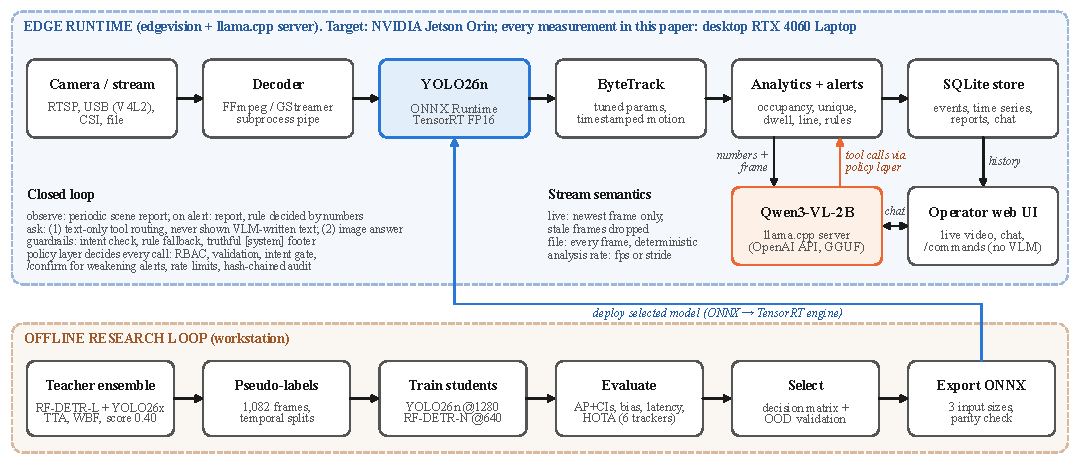
\includegraphics[width=\textwidth]{figures/fig_architecture.pdf}
\caption{System overview. Top: the on-device runtime; detections flow left to right, the VLM receives the live
analytics and frame and acts back on the analytics only through typed tool calls. Bottom: the offline research
loop that produces, evaluates, selects and exports the detector.}
\label{fig:arch}
\end{figure*}}

\subsection{Data and pseudo-labels}
\label{sec:data}
From the 300\,s, 59.94\,fps, $1280{\times}720$ video we sample one frame every 0.25\,s between 30\,s and 300\,s
(1,082 frames). Each frame is labelled by RF-DETR Large and YOLO26x (with test-time augmentation, $1280$\,px),
both at score $\geq 0.15$; their boxes are fused by WBF (IoU 0.55, equal weights, averaged scores) and fused
boxes with score $\geq 0.40$ are kept. The splits are contiguous in time so near-duplicate neighbouring frames
cannot leak across them: train 30--210\,s (\ImgsTrain{} frames, \BoxesTrain{} boxes), valid 210--255\,s
(\ImgsValid{}/\BoxesValid{}), test 255--300\,s (\ImgsTest{}/\BoxesTest{}). The first 30\,s are reserved for
tracking and never used for training (Fig.~\ref{fig:data}). The test split contains notably smaller people than
train (Fig.~\ref{fig:data}b), so test scores are not inflated by distribution overlap.

\figif{fig_dataset.pdf}{%
\begin{figure}[t]
\centering
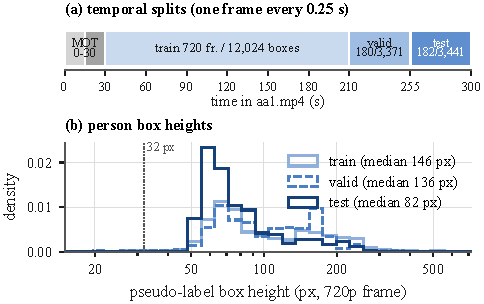
\includegraphics[width=\columnwidth]{figures/fig_dataset.pdf}
\caption{(a) Temporal use of \texttt{aa1}: tracking hold-out (0--15\,s tuning, 15--30\,s evaluation) and the
detection splits. (b) Pseudo-label box heights per split.}
\label{fig:data}
\end{figure}}

\subsection{Student training}
\yolo{} (COCO-pretrained, 2.5\,M parameters) is fine-tuned for 150 epochs at 1280\,px (AdamW, lr $10^{-3}$, cosine
schedule, batch 12). \rfdetr{} is fine-tuned at 640\,px for 80 epochs with EMA, cosine schedule and effective
batch 16 (lr $10^{-4}$, encoder $1.5{\times}10^{-4}$). An earlier 60-epoch step-schedule run reached the same
test AP and is not used further.

\subsection{Evaluation protocol}
All four models (both students, pretrained and fine-tuned) are scored with one script on every split.
\emph{COCO metrics}~\cite{lin2014coco}: \AP{}, \APf{}, \APs{}, AP by size, AR@300. \emph{Operating point}: the
best-F1 confidence threshold is chosen on \emph{valid} and frozen for test; we report P/R/F1 at IoU 0.5, FPPI
and the log-average miss rate (LAMR, FPPI $10^{-2}$--$10^{0}$)~\cite{dollar2012pedestrian}, and per-frame
counting MAE. \emph{Uncertainty}: 95\% bootstrap CIs over test images ($B{=}1000$)~\cite{efron1993bootstrap}
and paired bootstrap tests between models on identical resamples; with $B{=}1000$ a zero estimate is reported
as $p<0.001$. \emph{Overfitting}: the train--test gap of a fine-tuned model minus the same gap of its pretrained
counterpart, which saw no split and therefore measures split difficulty alone. \emph{Label bias}: test
predictions are re-scored against each teacher's labels alone (same 0.40 cut), since a student may inherit the
box conventions of its own family's teacher. \emph{Cross-check}: headline numbers are recomputed by code sharing
nothing with the evaluator (from-scratch 101-point AP, Hungarian matching, Ultralytics' validator, label
consistency, CI/test consistency; tracker re-runs and py-motmetrics).

\subsection{Tracking}
Tracking is evaluated on the unseen first 30\,s at the full frame rate (\GtFrames{} frames). Pseudo-GT tracks are
built by linking teacher detections with ByteTrack (activation 0.40, buffer \GtBuffer{} frames) and keeping
tracks of at least 0.25\,s (\GtTracks{} tracks). For each detector, ByteTrack parameters (score cut, NMS,
activation and high-score thresholds, buffer, IoU, confirmation frames) are grid-searched on 0--15\,s
(\GridSize{} configurations per detector) and reported on 15--30\,s. Because a GT linked by tracker $X$ favours
$X$, six trackers (SORT, ByteTrack, OC-SORT, C-BIoU, BoT-SORT, McByte; \texttt{trackers}
library~\cite{trackerslib}) are tuned by random search on 0--15\,s and scored on 15--30\,s against \emph{two}
pseudo-GTs built from the same teacher boxes, one linked by ByteTrack and one by OC-SORT.

\subsection{Model selection}
A decision matrix scores each fine-tuned student on six criteria relative to the best candidate (1\,=\,best):
test \AP{} under the fused labels (weight \MsWAp), the lower of its two single-teacher APs (\MsWBias), mean
held-out HOTA over the 12 tracker$\times$GT runs (\MsWHota), deployed latency (\MsWLat), GFLOPs (\MsWGflops) and
parameters (\MsWParams). The choice is re-checked under accuracy-only, speed-only, tracking-only, equal and
bias-aware weightings. The winner is exported to ONNX with the one-to-many head and external NMS (the variant
the latency study deploys) at $736{\times}1280$, $544{\times}960$ and $384{\times}640$, and each export is
re-scored on the test split through the runtime's own detector code.

\subsection{Edge system and closed loop}
\label{sec:edge}
\textbf{Stream ingest.} Files, RTSP/UDP/SRT/HTTP streams, V4L2 USB cameras and CSI cameras
(GStreamer \texttt{nvarguscamerasrc}) are decoded by an external FFmpeg~\cite{ffmpeg} or GStreamer process that
writes fixed-size BGR frames to a pipe. \emph{Live} sources keep only the newest frame (stale frames are dropped
and counted); \emph{files} are read without dropping, so file analysis is deterministic. The analysis rate is set
by resampling or by an exact frame stride.

\textbf{Detector and tracker.} The ONNX graph runs in ONNX Runtime with the TensorRT FP16 provider (engine cached
on disk), falling back to CUDA and CPU; no PyTorch is needed on the device. ByteTrack uses the tuned parameters
of the offline study, with the same score cut and class-agnostic NMS pre-filter; its lost-track buffer is defined
in seconds and the motion model uses real timestamps, so behaviour is consistent at any analysis rate and through
dropped live frames.

\textbf{Analytics and alerts.} Per frame we update occupancy, unique people (tracks $\geq$0.25\,s; an upper
bound, since a broken track counts twice), dwell, line crossings (foot point changes side, with hysteresis),
zones, loitering and image-plane speed. Rules such as \emph{occupancy $>$ 20 for 3\,s} fire alerts; events, 1-s
series, VLM reports and chat are stored in SQLite and served by a dependency-free web UI.

\textbf{VLM in the loop (evaluation-driven).} Qwen3-VL-2B (Q4\_K\_M GGUF) runs in a llama.cpp server with an
OpenAI-compatible API; one worker serves jobs by priority, so the per-frame loop never waits. Its role was fixed
by the experiments of Sec.~\ref{sec:vlm}. (i) \emph{Ask} is two-stage: stage~1 routes the question
\emph{text-only} (question, chat history, measurements) and may call \texttt{get\_history},
\texttt{get\_recent\_events}, \texttt{set\_alert}, \texttt{remove\_alert} or \texttt{set\_counting\_line} (up to
three rounds); stage~2 answers with the live frame, the updated measurements and the tool results, without tools.
A single-stage design with the frame attached produced many spurious tool calls (E3). Every change is validated,
logged and applied on the next frame, closing the loop from language back to measurement. (ii) \emph{On alert}
the VLM writes a scene report for the operator; the rule itself is decided by the detector numbers, because
yes/no verification by the VLM failed (E5). (iii) \emph{Observe}: a periodic JSON scene report (summary,
activities, anomalies and a risk level defined as visible physical danger, not crowd size). \emph{Guardrails}: a
deterministic intent check refuses tool arguments that contradict the request (e.g.\ a non-horizontal line for
``horizontal''); a rule-based executor performs unambiguous commands (remove all alerts, horizontal/vertical line
at a position) when the model did not; a system-generated footer states what actually changed, whatever the model
writes (it is not fed back into the chat history); and \texttt{/}commands give a VLM-free control path.
On the Jetson the plan is TensorRT FP16 at $544{\times}960$ with Qwen3-VL-2B on an Orin Nano 8\,GB and
$736{\times}1280$ with Qwen3-VL-4B on Orin NX/AGX, at a 15\,fps analysis rate.

%=====================================================================================================
\section{Experiments and Results}
All timings in this section are from a desktop with an RTX 4060 Laptop GPU (PyTorch path unless stated);
\ifHaveJetson the Jetson rows are marked explicitly.\else none were measured on a Jetson.\fi

\subsection{Detection}
\begin{table*}[t]
\centering
\caption{Detection on the test split (255--300\,s, \ImgsTest{} frames, \BoxesTest{} pseudo-GT boxes). F1 and count MAE
at the threshold chosen on valid (in parentheses); brackets: 95\% bootstrap CI. The last two columns re-score the
same predictions against a single teacher's labels (label-bias check; \LabelsRfL{} and \LabelsYx{} test boxes).}
\label{tab:det}
\footnotesize
\setlength{\tabcolsep}{3.6pt}
\begin{tabular}{lcccccccc|cc}
\toprule
 & \multicolumn{8}{c|}{Fused pseudo-labels (published)} & \multicolumn{2}{c}{\AP{} vs.\ single teacher} \\
Model & \AP{} [95\% CI] & \APf{} & \APs{} & \APsm{} & AR@300 & F1 (thr.) & LAMR$\downarrow$ & Count MAE$\downarrow$ & RF-DETR-L & YOLO26x \\
\midrule
\yolo{} pretrained & \ApYoloPt\ci{\ApLoYoloPt}{\ApHiYoloPt} & \ApFiftyYoloPt & \ApSeventyFiveYoloPt & \ApSmallYoloPt & \ArYoloPt & \FoneYoloPt{} (\ConfYoloPt) & \LamrYoloPt & \CountMaeYoloPt & \TbYoloPtRfL & \TbYoloPtYx \\
\yolo{} fine-tuned & \ApYoloFt\ci{\ApLoYoloFt}{\ApHiYoloFt} & \ApFiftyYoloFt & \ApSeventyFiveYoloFt & \ApSmallYoloFt & \ArYoloFt & \FoneYoloFt{} (\ConfYoloFt) & \LamrYoloFt & \CountMaeYoloFt & \TbYoloFtRfL & \TbYoloFtYx \\
\rfdetr{} pretrained & \ApRfPt\ci{\ApLoRfPt}{\ApHiRfPt} & \ApFiftyRfPt & \ApSeventyFiveRfPt & \ApSmallRfPt & \ArRfPt & \FoneRfPt{} (\ConfRfPt) & \LamrRfPt & \CountMaeRfPt & \TbRfPtRfL & \TbRfPtYx \\
\rfdetr{} fine-tuned & \ApRfFt\ci{\ApLoRfFt}{\ApHiRfFt} & \ApFiftyRfFt & \ApSeventyFiveRfFt & \ApSmallRfFt & \ArRfFt & \FoneRfFt{} (\ConfRfFt) & \LamrRfFt & \CountMaeRfFt & \TbRfFtRfL & \TbRfFtYx \\
\bottomrule
\end{tabular}
\end{table*}

Table~\ref{tab:det} and Fig.~\ref{fig:pr} summarise detection. Fine-tuning improves both students: \yolo{} by
\DeltaYoloFtPt{} \AP{} (CI \ci{\DeltaLoYoloFtPt}{\DeltaHiYoloFtPt}) and \rfdetr{} by \DeltaRfFtPt{}, whose
COCO-pretrained Nano model at 640\,px misses most of the small, distant pedestrians (\APsm{}~\ApSmallRfPt).
Fine-tuned \yolo{} leads fine-tuned \rfdetr{} by \DeltaFtFt{} \AP{} (paired CI
\ci{\DeltaLoFtFt}{\DeltaHiFtFt}, \PvalFtFt); the gap is concentrated at strict IoU (\APs{} \ApSeventyFiveYoloFt{}
vs.\ \ApSeventyFiveRfFt) and on small people (\APsm{} \ApSmallYoloFt{} vs.\ \ApSmallRfFt), while \APf{} is
close (\ApFiftyYoloFt{} vs.\ \ApFiftyRfFt). Part of this is resolution: \yolo{} sees the native 1280\,px width, and it is also far smaller
(\ParamsYoloFt\,M parameters, \GflopsYoloFt{} GFLOPs vs.\ \ParamsRfFt\,M and \GflopsRfFt{} for \rfdetr{} at its
inference resolution).

The two students fit the training frames differently. \yolo{} scores \ApTrainYoloFt{} / \ApValidYoloFt{} /
\ApTestYoloFt{} on train / valid / test; its train--test gap (\GapYoloFt) exceeds its pretrained counterpart's (\GapPtYoloFt) by \ExcessYoloFt{}, a measurable degree of
overfitting to the 720 training frames, yet it remains the best model on valid and test.
\rfdetr{} shows no excess gap (\ExcessRfFt). The low valid-optimal threshold of \yolo{} (\ConfYoloFt) maximises
F1 but over-counts (count MAE \CountMaeYoloFt{} vs.\ \CountMaeRfFt{} for \rfdetr{}); a counting deployment should
use a higher threshold. The independent cross-check passes \XcPass/\XcTotal{} detection checks (largest AP
deviation from pycocotools \XcApMaxDiff; Ultralytics' validator within \XcUltraDiff)\ifHaveTrackXc{} and
\XtPass/\XtTotal{} tracking checks\fi.

\begin{figure}[t]
\centering
\figif{fig_pr.pdf}{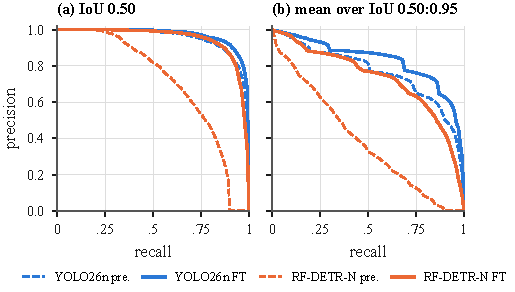
\includegraphics[width=\columnwidth]{figures/fig_pr.pdf}}
\caption{Test precision--recall curves (dashed: COCO-pretrained, solid: fine-tuned); the areas are the \APf{}
and \AP{} of Table~\ref{tab:det}.}
\label{fig:pr}
\end{figure}


\textbf{Label bias.} The last columns of Table~\ref{tab:det} re-score the test predictions against each teacher alone. Each
student scores best against its own family's teacher; under RF-DETR-Large-only labels the fine-tuned students
differ by only \TbGapRfL{} \AP{} (vs.\ \DeltaFtFt{} under fused labels), whereas under YOLO26x-only labels the gap
widens to \TbGapYx. The fused labels thus favour \yolo{}, and the detection ranking should be read as
``under these pseudo-labels''.


\textbf{Latency.} Table~\ref{tab:lat} and Fig.~\ref{fig:lat} time every inference variant end to end (BGR frame
in, boxes out, batch 1) and re-score it, so speed-ups that cost accuracy are visible. Uploading the uint8 frame
once and doing resize/normalisation on the GPU, a fused FP16 network and GPU NMS make \yolo{} \SpeedupYolo$\times$
faster than the stock path with unchanged AP; FP16, TorchScript and GPU pre-processing make \rfdetr{}
\SpeedupRf$\times$ faster. The NMS-free head of \yolo{} is the fastest variant but loses \NmsFreeApLoss{} \AP{} in
this crowded scene, so the deployed graph keeps the one-to-many head with NMS. At deployment \rfdetr{} remains
\LatRatio$\times$ slower.

\begin{table}[t]
\centering
\caption{Inference variants on the \ImgsTest{} test frames ($1280{\times}720$, RTX 4060 Laptop, batch 1, pre- and
post-processing included). Median / p90 latency in ms and test \AP{} of each variant.}
\label{tab:lat}
\footnotesize
\setlength{\tabcolsep}{2.8pt}
\begin{tabular}{lccc}
\toprule
Variant & Median & p90 & \AP{} \\
\midrule
\multicolumn{4}{l}{\emph{\yolo{}}} \\
\quad Ultralytics predict FP32 (stock) & \LatYoloBase & \LatPnYoloBase & \LatApYoloBase \\
\quad Ultralytics predict FP16 & \LatYoloHalf & \LatPnYoloHalf & \LatApYoloHalf \\
\quad NMS-free head FP16 & \LatYoloNmsFree & \LatPnYoloNmsFree & \LatApYoloNmsFree \\
\quad NMS-free + GPU pre-proc + fused FP16 & \LatYoloNmsFreeFast & \LatPnYoloNmsFreeFast & \LatApYoloNmsFreeFast \\
\quad \textbf{GPU pre-proc + fused FP16 + GPU NMS} & \textbf{\LatYoloDep} & \LatPnYoloDep & \LatApYoloDep \\
\multicolumn{4}{l}{\emph{\rfdetr{}}} \\
\quad predict FP32 (stock) & \LatRfBase & \LatPnRfBase & \LatApRfBase \\
\quad FP32 + TorchScript & \LatRfTs & \LatPnRfTs & \LatApRfTs \\
\quad FP16 & \LatRfHalf & \LatPnRfHalf & \LatApRfHalf \\
\quad FP16 + TorchScript & \LatRfHalfTs & \LatPnRfHalfTs & \LatApRfHalfTs \\
\quad \textbf{FP16 + TorchScript + GPU pre-proc} & \textbf{\LatRfDep} & \LatPnRfDep & \LatApRfDep \\
\bottomrule
\end{tabular}
\end{table}

\begin{figure}[t]
\centering
\figif{fig_latency.pdf}{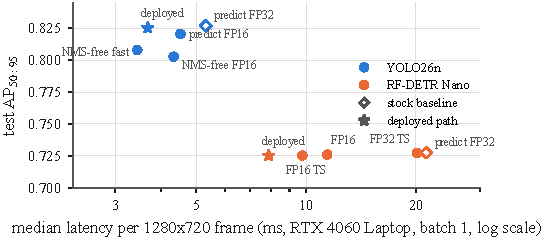
\includegraphics[width=\columnwidth]{figures/fig_latency.pdf}}
\caption{Latency vs.\ test \AP{} of the inference variants of Table~\ref{tab:lat} (stars: deployed paths).}
\label{fig:lat}
\end{figure}

\figif{fig_qualitative.png}{%
\begin{figure*}[t]
\centering
\includegraphics[width=0.86\textwidth]{figures/fig_qualitative.png}
\caption{Test frames: teacher pseudo-GT (left), fine-tuned \yolo{} (centre) and fine-tuned \rfdetr{} (right) at
their valid-optimal thresholds; titles give the number of boxes.}
\label{fig:qual}
\end{figure*}}

\subsection{Tracking}
Table~\ref{tab:track} reports ByteTrack on the held-out 15--30\,s with default and tuned parameters. With
default parameters the HOTA difference (\yolo{} minus \rfdetr) is \BtDefGap; \rfdetr{} needs a higher score cut
(\BtMinConfRf{} vs.\ \BtMinConfYolo), after which the difference is \BtTunGap{}---of the order of search
noise. The six-tracker comparison (Fig.~\ref{fig:track}) is more informative: \yolo{} scores higher in
\TcWinsAll{} of \TcPairs{} tracker$\times$GT combinations (\TcWinsOcGt/6 against the OC-SORT-linked GT,
\TcWinsBtGt/6 against the ByteTrack-linked GT), but never by more than \TcMaxGap{} HOTA. Within one detector the
six trackers span at most \TcSpreadBtGt{} (ByteTrack-GT) and \TcSpreadOcGt{} (OC-SORT-GT) HOTA, so the tracker
choice matters little in this scene. The absolute HOTA depends strongly on how the GT was linked (mean
\TcMeanYoloBtGt{} vs.\ \TcMeanYoloOcGt{} for \yolo), so models must only be compared under the same GT.

\begin{table}[t]
\centering
\caption{ByteTrack on the held-out 15--30\,s (pseudo-GT linked by ByteTrack; \BtGtIds{} GT identities). Tuned
parameters were selected on 0--15\,s.}
\label{tab:track}
\footnotesize
\setlength{\tabcolsep}{2.2pt}
\begin{tabular}{llccccccc}
\toprule
Detector & Params & HOTA & MOTA & IDF1 & DetA & AssA & IDSW & IDs \\
\midrule
\multirow{2}{*}{\yolo} & default & \BtHotaYoloDef & \BtMotaYoloDef & \BtIdfYoloDef & \BtDetaYoloDef & \BtAssaYoloDef & \BtIdswYoloDef & \BtIdsYoloDef \\
 & tuned & \BtHotaYoloTun & \BtMotaYoloTun & \BtIdfYoloTun & \BtDetaYoloTun & \BtAssaYoloTun & \BtIdswYoloTun & \BtIdsYoloTun \\
\midrule
\multirow{2}{*}{\rfdetr} & default & \BtHotaRfDef & \BtMotaRfDef & \BtIdfRfDef & \BtDetaRfDef & \BtAssaRfDef & \BtIdswRfDef & \BtIdsRfDef \\
 & tuned & \BtHotaRfTun & \BtMotaRfTun & \BtIdfRfTun & \BtDetaRfTun & \BtAssaRfTun & \BtIdswRfTun & \BtIdsRfTun \\
\bottomrule
\end{tabular}
\end{table}

\begin{figure}[t]
\centering
\figif{fig_tracking.pdf}{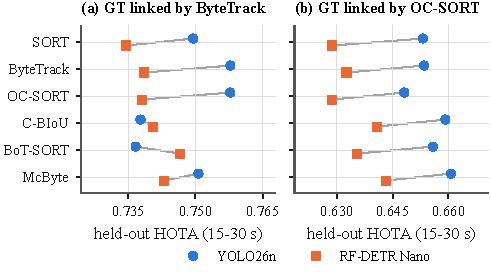
\includegraphics[width=\columnwidth]{figures/fig_tracking.pdf}}
\caption{Held-out HOTA of six trackers per detector, against pseudo-GTs linked by (a) ByteTrack and (b) OC-SORT.
Note the different x-ranges: GT linking shifts all scores.}
\label{fig:track}
\end{figure}

\textbf{Crowd analytics.} Over the first 30\,s, tracks of at least 0.25\,s give \AnUniqueYolo{} unique IDs
for \yolo{} (\AnOverYolo{} vs.\ \AnGtUnique{} in the pseudo-GT) and \AnUniqueRf{} for \rfdetr{}
(\AnOverRf); without the length filter \yolo{} produces \AnRawYolo{} raw IDs. Mean / max occupancy is
\AnMeanYolo{} / \AnMaxYolo{} and the median dwell \AnDwellMedYolo\,s. Unique IDs are an upper bound on people.

\subsection{Model selection and export}
Fig.~\ref{fig:sel} gives the decision matrix (raw values are in Tables~\ref{tab:det}, \ref{tab:lat} and
Fig.~\ref{fig:track}). \MsWinner{} wins with a weighted score of
\MsScoreYolo{} vs.\ \MsScoreRf; it is at least as good on \MsCritWins{} of \MsCritN{} criteria, including
the bias-aware AP and tracking (\MsTrackWinsYolo{} tracker$\times$GT wins), and the choice holds under all \MsNumAlt{} alternative
weightings (\rfdetr{} scores \MsAltAccRf{} accuracy-only, \MsAltSpeedRf{} speed-only, \MsAltTrackRf{}
tracking-only, \MsAltEqualRf{} equal, \MsAltBiasRf{} bias-aware, with \yolo{} at \MsScoreYolo). Re-scored on the test split through the runtime's own ONNX
detector, the $736{\times}1280$ export matches the PyTorch reference (\OnnxParityPt) within \OnnxParityDiff{}
\AP; the smaller Jetson inputs reach \OnnxMidAp{} ($544{\times}960$) and \OnnxLoAp{} ($384{\times}640$), losing
mainly small people (\APsm{} \OnnxHiApSmall, \OnnxMidApSmall, \OnnxLoApSmall\ifHaveEdge; Table~\ref{tab:edge}\fi).


\begin{figure}[t]
\centering
\figif{fig_selection.pdf}{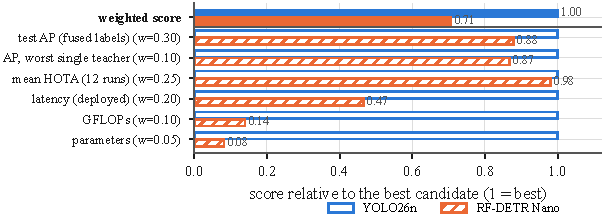
\includegraphics[width=\columnwidth]{figures/fig_selection.pdf}}
\caption{Normalised decision criteria (1 = best candidate) and weighted score.}
\label{fig:sel}
\end{figure}


%-----------------------------------------------------------------------------------------------------
\ifHaveEdge
\subsection{Streamed end-to-end pipeline}
We run the deployed runtime itself (FFmpeg decoder process $\rightarrow$ ONNX Runtime detector $\rightarrow$
ByteTrack $\rightarrow$ online analytics) on the tracking hold-out and score its tracks against the same
pseudo-GT (Table~\ref{tab:edge}, Fig.~\ref{fig:edge}). At the full frame rate the streamed pipeline reaches
held-out HOTA \EdHotaHiSOne{} (offline PyTorch study: \EdRefHota), confirming that export,
decoding and the online tracker reproduce the research result. Analysing every second or fourth frame (30 or
15\,fps, as planned for the Jetson) costs little HOTA (\EdHotaHiSTwo{} and \EdHotaHiSFour), because the tracker
uses real time steps; the smaller inputs cost more (\EdHotaMidSFour{} and \EdHotaLoSFour{} at 15\,fps),
mostly through missed small people (fewer unique IDs). These runs used the \texttt{\EdProvider} back-end of ONNX
Runtime on the desktop CPU, so their latencies characterise the software path, not TensorRT on a Jetson;
tracking and analytics together cost about \EdTrkMsHiSOne{} and \EdAnaMsHiSOne\,ms per frame.
\ifHaveEdgeLive
Read as a real-time RTSP camera at full rate (GPU PyTorch back-end), the runtime analysed
\EdLiveFrames{} of about \EdLivePublished{} frames at \EdLiveFps\,fps, dropping stale ones by design.
\fi

\begin{table}[t]
\centering
\caption{Deployed runtime per ONNX input size. \AP: export re-scored on the detection test split. Tracking on
the 15--30\,s hold-out (file source); ``Unique'' = tracks $\geq$0.25\,s over 0--30\,s (pseudo-GT in parentheses).
Latency: median ms per frame, ONNX Runtime \texttt{\EdProvider} on the desktop.}
\label{tab:edge}
\footnotesize
\setlength{\tabcolsep}{2.3pt}
\begin{tabular}{lccccccc}
\toprule
Input $H$, rate & \AP & HOTA & MOTA & IDF1 & Unique (GT) & Det. & Loop \\
\midrule
736, \EdFpsHiSOne\,fps & \OnnxHiAp & \EdHotaHiSOne & \EdMotaHiSOne & \EdIdfHiSOne & \EdUniqueHiSOne{} (\EdGtUniqueHiSOne) & \EdDetMsHiSOne & \EdLoopMsHiSOne \\
736, \EdFpsHiSTwo\,fps & \OnnxHiAp & \EdHotaHiSTwo & \EdMotaHiSTwo & \EdIdfHiSTwo & \EdUniqueHiSTwo{} (\EdGtUniqueHiSTwo) & \EdDetMsHiSTwo & \EdLoopMsHiSTwo \\
736, \EdFpsHiSFour\,fps & \OnnxHiAp & \EdHotaHiSFour & \EdMotaHiSFour & \EdIdfHiSFour & \EdUniqueHiSFour{} (\EdGtUniqueHiSFour) & \EdDetMsHiSFour & \EdLoopMsHiSFour \\
544, \EdFpsMidSFour\,fps & \OnnxMidAp & \EdHotaMidSFour & \EdMotaMidSFour & \EdIdfMidSFour & \EdUniqueMidSFour{} (\EdGtUniqueMidSFour) & \EdDetMsMidSFour & \EdLoopMsMidSFour \\
384, \EdFpsLoSFour\,fps & \OnnxLoAp & \EdHotaLoSFour & \EdMotaLoSFour & \EdIdfLoSFour & \EdUniqueLoSFour{} (\EdGtUniqueLoSFour) & \EdDetMsLoSFour & \EdLoopMsLoSFour \\
\midrule
Offline study & \OnnxParityPt & \EdRefHota & \multicolumn{5}{l}{(PyTorch FP16, every frame)} \\
\bottomrule
\end{tabular}
\end{table}

\begin{figure}[t]
\centering
\figif{fig_edge.pdf}{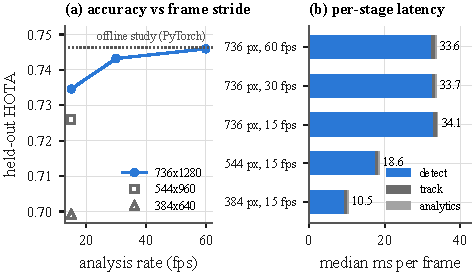
\includegraphics[width=\columnwidth]{figures/fig_edge.pdf}}
\caption{Deployed runtime: (a) held-out HOTA vs.\ analysis rate and input size; (b) median per-stage latency
(desktop CPU ONNX Runtime, not TensorRT).}
\label{fig:edge}
\end{figure}
\fi

%-----------------------------------------------------------------------------------------------------
\ifHaveVLM
\subsection{VLM in the loop}
\label{sec:vlm}
\ifHaveVLMEOne
\textbf{E1: count grounding.} On the \EoFrames{} test frames (pseudo-GT counts \EoGtMin--\EoGtMax{} people), we
compare the detector alone (ONNX, valid-optimal threshold) with the VLM under four prompts
(Fig.~\ref{fig:vlmcount}). From the image alone Qwen3-VL-2B undercounts severely
(MAE \EoMaeB, bias \EoBiasB). Adding the deployed system prompt already helps (\EoMaeBsys), and with the detector
count in the context its error falls to \EoMaeC{} (paired bootstrap, image-only minus grounded: \EoDeltaBC,
CI \ci{\EoDeltaLoBC}{\EoDeltaHiBC}, \EoPvalBC). However, the grounded VLM returns the detector's number in a
fraction \EoCopyC{} of frames, and the text-only control behaves identically: grounding \emph{transfers} the
detector's accuracy (and its bias, \EoBiasA) rather than improving on it, so counts are always taken from the
analytics.
\fi

\ifHaveVLMETwo
\textbf{E2: zero-shot attributes.} On the held-out campus test tracks, the VLM's zero-shot uniform/gender votes
(three crops per track) are compared with the trained linear probes of Sec.~\ref{sec:campus}. Per track,
dress accuracy is \EtVlmAccUni{} \ci{\EtVlmLoUni}{\EtVlmHiUni} (Wilson CI~\cite{wilson1927}) for the VLM vs.\ \EtProbeAccUni{} for the probe
(coverage \EtVlmCovUni{} vs.\ \EtProbeCovUni), and gender \EtVlmAccGen{} vs.\ \EtProbeAccGen; on the tracks both
answered, an exact McNemar test~\cite{mcnemar1947} gives \EtMcPUni{} and \EtMcPGen. Zero-shot description is thus
competitive with trained probes here.
\fi

\ifHaveVLMEThree
\textbf{E3: tool-call reliability.} We send \EthNTool{} operator utterances that require exactly one tool call
with determined arguments and \EthNNoTool{} that require none (Table~\ref{tab:tools}). In the original
single-stage design (frame attached, tools offered) selection on tool utterances is high (\EthSelToolFrame) and
all arguments are valid JSON, but exact arguments match in only \EthArgFrame{} of cases and the model calls tools
on \EthFpFrame{} of the utterances that need none; text-only, that false-call rate falls to \EthFpText.
\ifHaveVLMEThreeB
The redesigned two-stage agent (text-only routing, a clearer \texttt{set\_alert} schema, guardrails) reaches
selection \EtbSel, exact arguments \EtbArg{} and a false-call rate of \EtbFp{} on the same utterances, at
\EtbReq{} requests and \EtbLat\,s median per turn. The guardrails did not fire on this set (\EtbFallback{}
fallback actions; model-only selection \EtbMoSel, arguments \EtbMoArg), so the gain comes from routing and schema;
because the schema also changed, the two effects are not separated.
\fi
\fi

\ifHaveVLMEFive
\textbf{E5: alert verification.} On \EvN{} test frames each, we pose a true occupancy alert (threshold below the
pseudo-GT count) and a fabricated one (threshold and claimed value above it, as if the detector over-counted).
Shown the measured value, the VLM confirms every true alert (sensitivity \EvSensInformed) but also every fabricated
one (specificity \EvSpecInformed\ci{\EvSpecLoInformed}{\EvSpecHiInformed}); from the image alone it is below chance
(sensitivity \EvSensBlind, specificity \EvSpecBlind, balanced accuracy \EvBalBlind). A 2B VLM cannot audit a
count it cannot make, so the deployed default writes a scene report on alert and leaves the decision to the
numbers.
\fi

\ifHaveVLMEFour
\textbf{E4: latency.} On the desktop GPU (llama.cpp Vulkan, prompt cache disabled), a scene report takes a median
of \EfEImgXs, \EfEImgM{} and \EfEImgL\,s at image sides 448, 896 and 1280\,px, a text answer \EfEText\,s and a
tool-call turn \EfETool\,s (prompt \EfTokImgM{} tokens at 896\,px, decode \EfDecImgM{} tokens/s). VLM jobs run
asynchronously and never block the per-frame loop.
\fi

\ifHaveVLMEOne
\begin{figure}[t]
\centering
\figif{fig_vlm_counting.pdf}{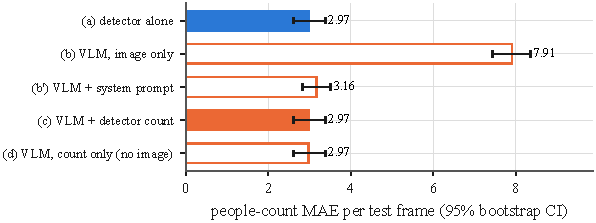
\includegraphics[width=\columnwidth]{figures/fig_vlm_counting.pdf}}
\caption{E1: counting MAE per condition (95\% bootstrap CIs over frames).}
\label{fig:vlmcount}
\end{figure}
\fi

\ifHaveVLMEThree
\begin{table}[t]
\centering
\caption{E3: tool-call reliability of Qwen3-VL-2B (\EthNTool{} tool and \EthNNoTool{} no-tool utterances):
single-stage agent with / without the frame vs.\ the deployed two-stage agent with guardrails (E3b).}
\label{tab:tools}
\scriptsize
\setlength{\tabcolsep}{2.2pt}
\begin{tabular}{lccc}
\toprule
 & \multicolumn{2}{c}{Single stage} & Two-stage \\
Metric & with frame & text only & (deployed) \\
\midrule
Selection, all [95\% CI] & \EthSelFrame\ci{\EthSelLoFrame}{\EthSelHiFrame} & \EthSelText\ci{\EthSelLoText}{\EthSelHiText} & \ifHaveVLMEThreeB\EtbSel\ci{\EtbSelLo}{\EtbSelHi}\else--\fi \\
Selection, tool utterances & \EthSelToolFrame & \EthSelToolText & \ifHaveVLMEThreeB\EtbSelTool\else--\fi \\
Exact arguments [95\% CI] & \EthArgFrame\ci{\EthArgLoFrame}{\EthArgHiFrame} & \EthArgText\ci{\EthArgLoText}{\EthArgHiText} & \ifHaveVLMEThreeB\EtbArg\ci{\EtbArgLo}{\EtbArgHi}\else--\fi \\
Lenient arguments & \EthArgLenFrame & \EthArgLenText & \ifHaveVLMEThreeB\EtbArgLen\else--\fi \\
False tool calls (no-tool) & \EthFpFrame & \EthFpText & \ifHaveVLMEThreeB\EtbFp\else--\fi \\
Missed tool calls & \EthMissFrame & \EthMissText & \ifHaveVLMEThreeB\EtbMiss\else--\fi \\
Median latency (s) & \EthLatFrame & \EthLatText & \ifHaveVLMEThreeB\EtbLat\else--\fi \\
\bottomrule
\end{tabular}
\end{table}
\fi

\ifHaveDemo
\textbf{Closed-loop session.} We recorded a \DmDuration\,s session on a live RTSP stream (MediaMTX, real time,
analysed at \DmRate\,fps; \DmFrames{} frames, \DmDropped{} stale frames dropped, median loop \DmLoopMs\,ms on the
desktop GPU), with the operator acting only through the HTTP chat API (Fig.~\ref{fig:demo}). Of \DmCtl{} control
requests, the model executed \DmCtlModel{} itself (setting an occupancy alert, reading history, removing all
alerts); for ``make the counting line horizontal'' it produced contradicting arguments \DmLineFails{} times, the
intent check refused each, and the rule-based executor set the line. The alert fired (occupancy \DmAlertValue{}
$>$ \DmAlertThr) and received a scene report after \DmAlertCtxLat\,s; the median chat latency was
\DmChatMed\,s. The free-text answers were not always reliable (one repeated a stale count from an earlier turn),
which is why counts are read from \texttt{/stats} or the UI and state changes from the system footer.
\fi

\ifHaveDemo
\begin{figure}[t]
\centering
\figif{fig_demo.jpg}{\includegraphics[width=0.8\columnwidth]{figures/fig_demo.jpg}}
\caption{End of the recorded closed-loop session: the counting line was made horizontal by chat (rule-based
fallback after the model's arguments were refused); status bar shows live occupancy and unique tracks.}
\label{fig:demo}
\end{figure}
\fi
\fi

%-----------------------------------------------------------------------------------------------------
\ifHaveHeldout
\subsection{Held-out scene: a test-only video}
\label{sec:heldout}
To test whether the conclusions transfer beyond \texttt{aa1}, we evaluate on a second video that is used
\emph{only} for testing: \HoDur\,s of a tree-lined campus road filmed from a fixed position ($1920{\times}1080$,
variable frame rate, mean \HoFps\,fps, \HoFrames{} frames). Nothing is trained, tuned or selected on it: the models are
the aa1 checkpoints, the operating thresholds are the aa1-valid ones, and the tracker parameters are the ones
selected on aa1. The teacher recipe of Sec.~\ref{sec:data} labels \HoImgs{} frames sampled every 0.25\,s
(\HoBoxes{} boxes, \HoPerFrame{} people per frame, median height \HoHeightMed\,px) and, for tracking, every frame
(\HoGtIds{} pseudo-GT identities). Frames 0.25\,s apart are strongly correlated, so CIs use a moving-block bootstrap
with 10\,s blocks (\HoBlock{} frames); the counting line was fixed from one frame before any result was computed.

\begin{table}[t]
\centering
\caption{Held-out video, detection (\HoImgs{} frames). $\Delta$: change from the aa1 test split (Table~\ref{tab:det}).
$R_{32\text{--}64}$: recall of people 32--64\,px tall and F1, both at the threshold frozen from aa1-valid. Brackets:
95\% block-bootstrap CI. Last columns: \AP{} against a single teacher's labels.}
\label{tab:heldout}
\footnotesize
\setlength{\tabcolsep}{1.15pt}
\begin{tabular}{lcccccc}
\toprule
Model & \AP{} [95\% CI] & $\Delta$ & $R_{32\text{--}64}$ & F1 & RF-L & Y26x \\
\midrule
\yolo{} pre. & \textbf{\HoApYoloPt}\ci{\HoApLoYoloPt}{\HoApHiYoloPt} & \HoDropYoloPt & \textbf{\HoRecSmallYoloPt} & \textbf{\HoFoneYoloPt} & \textbf{\HoTbRfLYoloPt} & \textbf{\HoTbYxYoloPt} \\
\yolo{} FT & \HoApYoloFt\ci{\HoApLoYoloFt}{\HoApHiYoloFt} & \HoDropYoloFt & \HoRecSmallYoloFt & \HoFoneYoloFt & \HoTbRfLYoloFt & \HoTbYxYoloFt \\
\rfdetr{} pre. & \HoApRfPt\ci{\HoApLoRfPt}{\HoApHiRfPt} & \HoDropRfPt & \HoRecSmallRfPt & \HoFoneRfPt & \HoTbRfLRfPt & \HoTbYxRfPt \\
\rfdetr{} FT & \HoApRfFt\ci{\HoApLoRfFt}{\HoApHiRfFt} & \HoDropRfFt & \HoRecSmallRfFt & \HoFoneRfFt & \HoTbRfLRfFt & \HoTbYxRfFt \\
\bottomrule
\end{tabular}
\end{table}

\textbf{Detection: the ranking reverses.} Fine-tuned \yolo{}, the aa1 winner, drops from \ApYoloFt{} to \HoApYoloFt{} \AP{}
($\Delta$\,=\,\HoDropYoloFt) and falls \emph{below its own COCO-pretrained weights} (paired $\Delta$\,=\,\HoDeltaYoloFtPt,
CI\ci{\HoDeltaLoYoloFtPt}{\HoDeltaHiYoloFtPt}, \HoPvalYoloFtPt) and below fine-tuned \rfdetr{} ($\Delta$\,=\,\HoDeltaFtFt,
CI\ci{\HoDeltaLoFtFt}{\HoDeltaHiFtFt}), whose fine-tuning still helps (\HoDeltaRfFtPt{} over its pretrained model).
The best detector on the new scene is the pretrained \yolo{} (Table~\ref{tab:heldout}, Fig.~\ref{fig:heldout}a). The
loss is concentrated on small people: at the frozen threshold the fine-tuned \yolo{} finds \HoRecSmallYoloFt{} of the
people 32--64\,px tall (pretrained weights: \HoRecSmallYoloPt; Fig.~\ref{fig:heldout}b) and makes
\HoFppiYoloFt{} false positives per frame (pretrained: \HoFppiYoloPt); in the audited frames about half of them are
bins, benches and tree trunks and most of the rest are poorly localised or duplicate boxes on people.
This is the scene overfitting that the excess train--test gap on aa1 (\ExcessYoloFt) hinted at; \rfdetr{}, which showed
no excess gap, transfers better. The ranking is the same under either teacher's labels alone, although the teachers
agree less on this scene (RF-DETR-L boxes score \HoTeacherAgree{} \AP{} against YOLO26x labels).

\textbf{Label audit.} Because every number here is agreement with the teachers, we inspected the disagreements on
\HoAuFrames{} random frames (crops judged by the authors' AI assistant): \HoAuLabPerson/\HoAuLabN{} randomly drawn
labels are people (\HoAuLabRate\ci{\HoAuLabLo}{\HoAuLabHi}), and so are \HoAuFnPerson/\HoAuFnN{} labels that a model
missed (\HoAuFnRate), so the misses are real. Of the \HoAuFpN{} model detections far from any label,
\HoAuFpPerson{} are people the teachers missed (\HoAuFpRate\ci{\HoAuFpLo}{\HoAuFpHi}); the rest are bins, benches and
trees. Crediting every audited label error to the models changes no F1 by more than \HoAuMaxFoneShift, so the
reversal is not a pseudo-label artefact.

\begin{table}[t]
\centering
\caption{Held-out video, ByteTrack with the aa1 parameters (\HoFrames{} frames, \HoGtIds{} pseudo-GT identities;
default ByteTrack parameters in parentheses). Crossings: events on the counting line, F1 of matching the
\HoAnGtCross{} pseudo-GT events ($\pm$1\,s, same direction).}
\label{tab:hotrack}
\footnotesize
\setlength{\tabcolsep}{1.9pt}
\begin{tabular}{lcccccc}
\toprule
Detector & HOTA & MOTA & IDF1 & IDSW & Cross. & Cross. F1 \\
\midrule
\yolo{} FT & \HoBtHotaYoloFtTun{} (\HoBtHotaYoloFtDef) & \HoBtMotaYoloFtTun & \HoBtIdfYoloFtTun & \HoBtIdswYoloFtTun & \HoAnCrossYoloFt & \HoAnCrossFoneYoloFt \\
\rfdetr{} FT & \HoBtHotaRfFtTun{} (\HoBtHotaRfFtDef) & \HoBtMotaRfFtTun & \HoBtIdfRfFtTun & \HoBtIdswRfFtTun & \HoAnCrossRfFt & \HoAnCrossFoneRfFt \\
\yolo{} pre. & \textbf{\HoBtHotaYoloPtTun}{} (\HoBtHotaYoloPtDef) & \textbf{\HoBtMotaYoloPtTun} & \textbf{\HoBtIdfYoloPtTun} & \textbf{\HoBtIdswYoloPtTun} & \textbf{\HoAnCrossYoloPt} & \textbf{\HoAnCrossFoneYoloPt} \\
\bottomrule
\end{tabular}
\end{table}

\figif{fig_heldout.pdf}{%
\begin{figure*}[t]
\centering
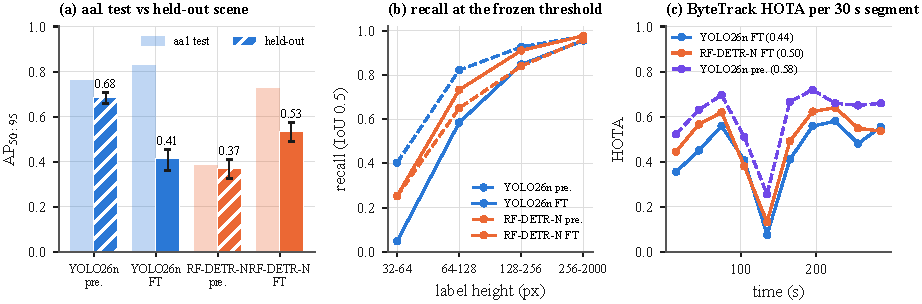
\includegraphics[width=\textwidth]{figures/fig_heldout.pdf}
\caption{Held-out video (test only). (a) \AP{} on the aa1 test split (light) and on the held-out video (dark, 95\%
block-bootstrap CI); hatched: COCO-pretrained. (b) Recall by label height at the thresholds frozen from aa1.
(c) ByteTrack HOTA per 30\,s segment with the aa1 parameters (whole-video HOTA in the legend); the dip near 135\,s is a
stretch with almost nobody in view.}
\label{fig:heldout}
\end{figure*}}

\textbf{Tracking and analytics.} With the frozen parameters, fine-tuned \rfdetr{} tracks better than fine-tuned \yolo{}
(Table~\ref{tab:hotrack}): it wins \HoSegWinsRf{} of \HoSegs{} 30\,s segments (Wilcoxon $p=\HoSegPFtFt$) and
\HoTcWinsRf{} of \HoTcPairs{} tracker$\times$GT combinations of the six-tracker comparison, the reverse of aa1. The
pretrained \yolo{}, never tuned for tracking, is best and wins \HoSegWinsPt/\HoSegs{} segments against \rfdetr{}
($p=\HoSegPPtRf$). Absolute HOTA (\HoBtHotaYoloFtTun--\HoBtHotaYoloPtTun{} vs.\ \BtHotaYoloTun{} and \BtHotaRfTun{} on the aa1 hold-out) is depressed by distant people that the
students do not detect: mean occupancy is \HoAnOccYoloFt, \HoAnOccRfFt{} and \HoAnOccYoloPt{} vs.\ \HoAnGtOcc{} in the
pseudo-GT. Near the camera the analytics are more robust: the pretrained \yolo{} recovers the counting-line events
with F1 \HoAnCrossFoneYoloPt{} (count error \HoAnCrossErrYoloPt). Unique-ID counts are not a usable metric here:
\rfdetr{} reports \HoAnUniqueRfFt{} people vs.\ \HoAnGtUnique{} in the pseudo-GT only because track fragmentation
(\HoBtIdswRfFtTun{} ID switches) and missed distant people cancel.
\ifHaveHeldoutEdge
The deployed runtime with the fine-tuned \yolo{} ONNX model inherits the detector's weakness: HOTA
\HoEdHotaHiSOne{} at the full rate (offline: \HoEdRefHota), \HoEdHotaHiSFour{} at 15\,fps and \HoEdHotaMidSFour{} with
the $544{\times}960$ Jetson input. This test also exposed a runtime bug that the constant-rate aa1 video could not:
without an explicit output rate, FFmpeg's raw-video output resampled the variable-frame-rate file to a constant rate
(\HoVfrDelivered{} instead of \HoVfrFrames{} frames), and file timestamps computed as index\,/\,mean fps drifted by up
to \HoVfrTsErr\,s. Frames are now passed through unchanged and stamped with their container timestamps; this raised
the full-rate HOTA from \HoVfrHotaBefore{} to \HoEdHotaHiSOne{} and left every aa1 number unchanged.
\fi
\fi

%-----------------------------------------------------------------------------------------------------
\subsection{Campus case study}
\label{sec:campus}
To test transfer to a new domain we analysed two $\sim$200\,s, 1080p phone videos of a university campus. Nothing
here needs real time, so the teacher detector YOLO26x at 1280\,px is used with BoT-SORT (ReID and motion
compensation); broken tracks are re-joined offline when motion, box size, colours and predicted attributes agree.
Two attribute heads (uniform vs.\ non-uniform, gender) are logistic-regression probes on DINOv2 features of the
RF-DETR-L backbone plus colour histograms, trained on 200 hand-labelled tracks and evaluated on 100 disjoint
random tracks; they abstain when the mean probability is within 0.35--0.65. Table~\ref{tab:campus} and
Fig.~\ref{fig:campus} summarise the outputs. Held out per person, the probes reach \PrUniAcc{}
\ci{\PrUniLo}{\PrUniHi} accuracy for dress (\PrUniCorrect/\PrUniAnswered, coverage \PrUniCov) and \PrGenAcc{}
\ci{\PrGenLo}{\PrGenHi} for gender (\PrGenCorrect/\PrGenAnswered, coverage \PrGenCov). The hand labels were
produced by the authors' AI assistant from the crops, not by independent annotators, and gender is predicted from
appearance (the uniform is gendered); it is reported only as an aggregate.

\begin{table}[t]
\centering
\caption{Campus case study (YOLO26x + BoT-SORT + stitching; attributes over people with a usable crop).}
\label{tab:campus}
\footnotesize
\setlength{\tabcolsep}{2.4pt}
\begin{tabular}{lcc}
\toprule
 & video 1 & video 2 \\
\midrule
Track IDs $\rightarrow$ kept $\rightarrow$ people & \CpOneRaw{} $\rightarrow$ \CpOneKept{} $\rightarrow$ \CpOnePeople & \CpTwoRaw{} $\rightarrow$ \CpTwoKept{} $\rightarrow$ \CpTwoPeople \\
In frame, mean / peak & \CpOneMean{} / \CpOnePeak & \CpTwoMean{} / \CpTwoPeak \\
Crossings (R$\rightarrow$L/L$\rightarrow$R) & \CpOneCross{} (\CpOneCrossRl/\CpOneCrossLr) & \CpTwoCross{} (\CpTwoCrossRl/\CpTwoCrossLr) \\
Median time in view (s) & \CpOneDwell & \CpTwoDwell \\
Gender m / f / unsure & \CpOneMale{} / \CpOneFemale{} / \CpOneGUnsure & \CpTwoMale{} / \CpTwoFemale{} / \CpTwoGUnsure \\
Dress unif. / non-u. / unsure & \CpOneUniform{} / \CpOneNonUniform{} / \CpOneDUnsure & \CpTwoUniform{} / \CpTwoNonUniform{} / \CpTwoDUnsure \\
\bottomrule
\end{tabular}
\end{table}

\begin{figure}[t]
\centering
\figif{fig_campus.pdf}{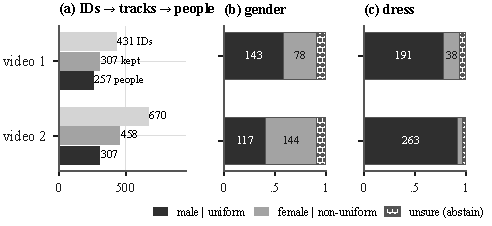
\includegraphics[width=\columnwidth]{figures/fig_campus.pdf}}
\caption{Campus case study: (a) counting funnel from raw track IDs to stitched people; (b, c) attribute shares.}
\label{fig:campus}
\end{figure}

%=====================================================================================================
\section{Discussion and Limitations}
\textbf{Pseudo-GT is not human GT.} Every detection and tracking number measures agreement with a larger teacher
ensemble. The label-bias analysis shows that the \yolo{} advantage shrinks to \TbGapRfL{} \AP{} under
RF-DETR-Large-only labels, and the mean tracking HOTA of \yolo{} moves from \TcMeanYoloBtGt{} to \TcMeanYoloOcGt{} when only the GT
linking changes. Relative comparisons
under one GT are meaningful; absolute values are not accuracy against reality. A visual audit on the held-out video
(Sec.~\ref{sec:heldout}) found the labels precise (\HoAuLabRate{} of sampled labels are people) and the
model--label disagreements dominated by genuine model errors, but it was done by an AI assistant from crops and covers
only \HoAuFrames{} frames.

\textbf{In-domain selection does not transfer.} The students were trained on one 5-minute video, and the aa1 test
split shares its scene. On the held-out video the selected model is the worst fine-tuned detector and is beaten by its
own pretrained weights (Sec.~\ref{sec:heldout}), so an in-domain decision matrix only answers ``which model for
\emph{this} camera''. The aa1 overfitting diagnosis (excess train--test gap) predicted which student transfers worse;
we recommend adding a held-out-scene criterion to the selection, re-fine-tuning per site from teacher labels (the
pipeline makes this cheap), or deploying the pretrained detector on cameras without site-specific labels. Two scenes
are still few, and bootstrap CIs capture frame sampling, not scene variation. The campus case study videos were
analysed with the teacher detector.

\textbf{Image-plane analytics.} Line crossings, flow and speeds are computed in image coordinates and include
camera motion for a handheld camera. Unique track IDs are an upper bound on unique people; the campus
re-joining reduces but does not remove double counting.

\textbf{Hand labels.} The campus attribute labels were produced by an AI assistant from crops, not by
independent annotators.

\textbf{What a small VLM is for.} A 2B VLM must not be trusted for counts (E1) or yes/no verdicts on measured
quantities (E5), and its free text can restate stale numbers. Its value here is description (scene and alert
reports, zero-shot attributes, E2) and natural-language control, and the latter became dependable only with
text-only routing plus deterministic guardrails: intent checks, rule-based fallbacks, a truthful state footer
and a VLM-free command path. Each of these was added in response to a measured or observed failure.

\textbf{Jetson.} \ifHaveJetson Jetson measurements are reported where marked.\else The Jetson deployment is
designed and packaged (three ONNX input sizes, TensorRT engine cache, CSI input, llama.cpp CUDA build, service
files), but all timings here are desktop measurements; on-device benchmarks are future work.\fi

%=====================================================================================================
\section{Conclusion}
We built and evaluated a complete path from an unlabelled video to a closed-loop crowd-analytics system. Under a
protocol with CIs, paired tests, a label-bias check and independent metric re-implementations, fine-tuned \yolo{}
is the better deployment choice than \rfdetr{} for the training scene (\ApYoloFt{} vs.\ \ApRfFt{} \AP, at least as
good for tracking, \LatRatio$\times$ faster), although its detection margin depends partly on the teacher. A test-only
second scene reverses this (\HoApYoloFt{} vs.\ \HoApRfFt, pretrained \yolo{} \HoApYoloPt): scene-specific
fine-tuning of a nano model must be validated on a held-out scene before it is deployed elsewhere. The deployed runtime
reproduces the offline tracking accuracy when streamed, and a small VLM adds scene descriptions and
natural-language reconfiguration as a describer and router, while counts, alert decisions and the record of
changes stay deterministic. Future work: Jetson benchmarks, human-annotated labels, more scenes, and multi-scene fine-tuning. All numbers are
generated from the result files (\texttt{paper/make\_numbers.py}).

% \balance  (columns on the last page are already nearly equal; balance overfilled the left column)
\bibliographystyle{IEEEtran}
\bibliography{refs}

\end{document}
